%\begin{frame} [fragile] 
%\frametitle{Redirect} 
%Il  campo uilizzato per l'inserimento dei dati sarà \textbf{Internet 
%Header+ 64 bits}. La quantità di dati esfiltrabili tramite questo messaggio 
%sarà pari a \textbf{9 byte}. 
%\begin{center} 
%{\scriptsize 
%\begin{bytefield}[bitwidth=1.1em]{32} 
%        %\bitbox{8}{0} & \bitbox{8}{1} & \bitbox{8}{2} & \bitbox{8}{3} \\
%        \bitheader{0-31} \\
%        \bitbox{8}{Type=5 (1 byte)} & \bitbox{8}{Code=0-3 (1 byte)} & \bitbox{16}{Checksum (2 byte)} \\
%        \bitbox{32}{Gateway Internet Address (4 byte)} \\
%        \bitbox{32}{Internet Header + 64 bits of Original Datagram ($\geq$ 21B)} 
%\end{bytefield}
%\captionof{figure}{Struttura del pacchetto \textbf{ICMPv4 Redirect}}
%} \end{center} 
%\end{frame} 
%\begin{frame}
%%\begin{figure}
%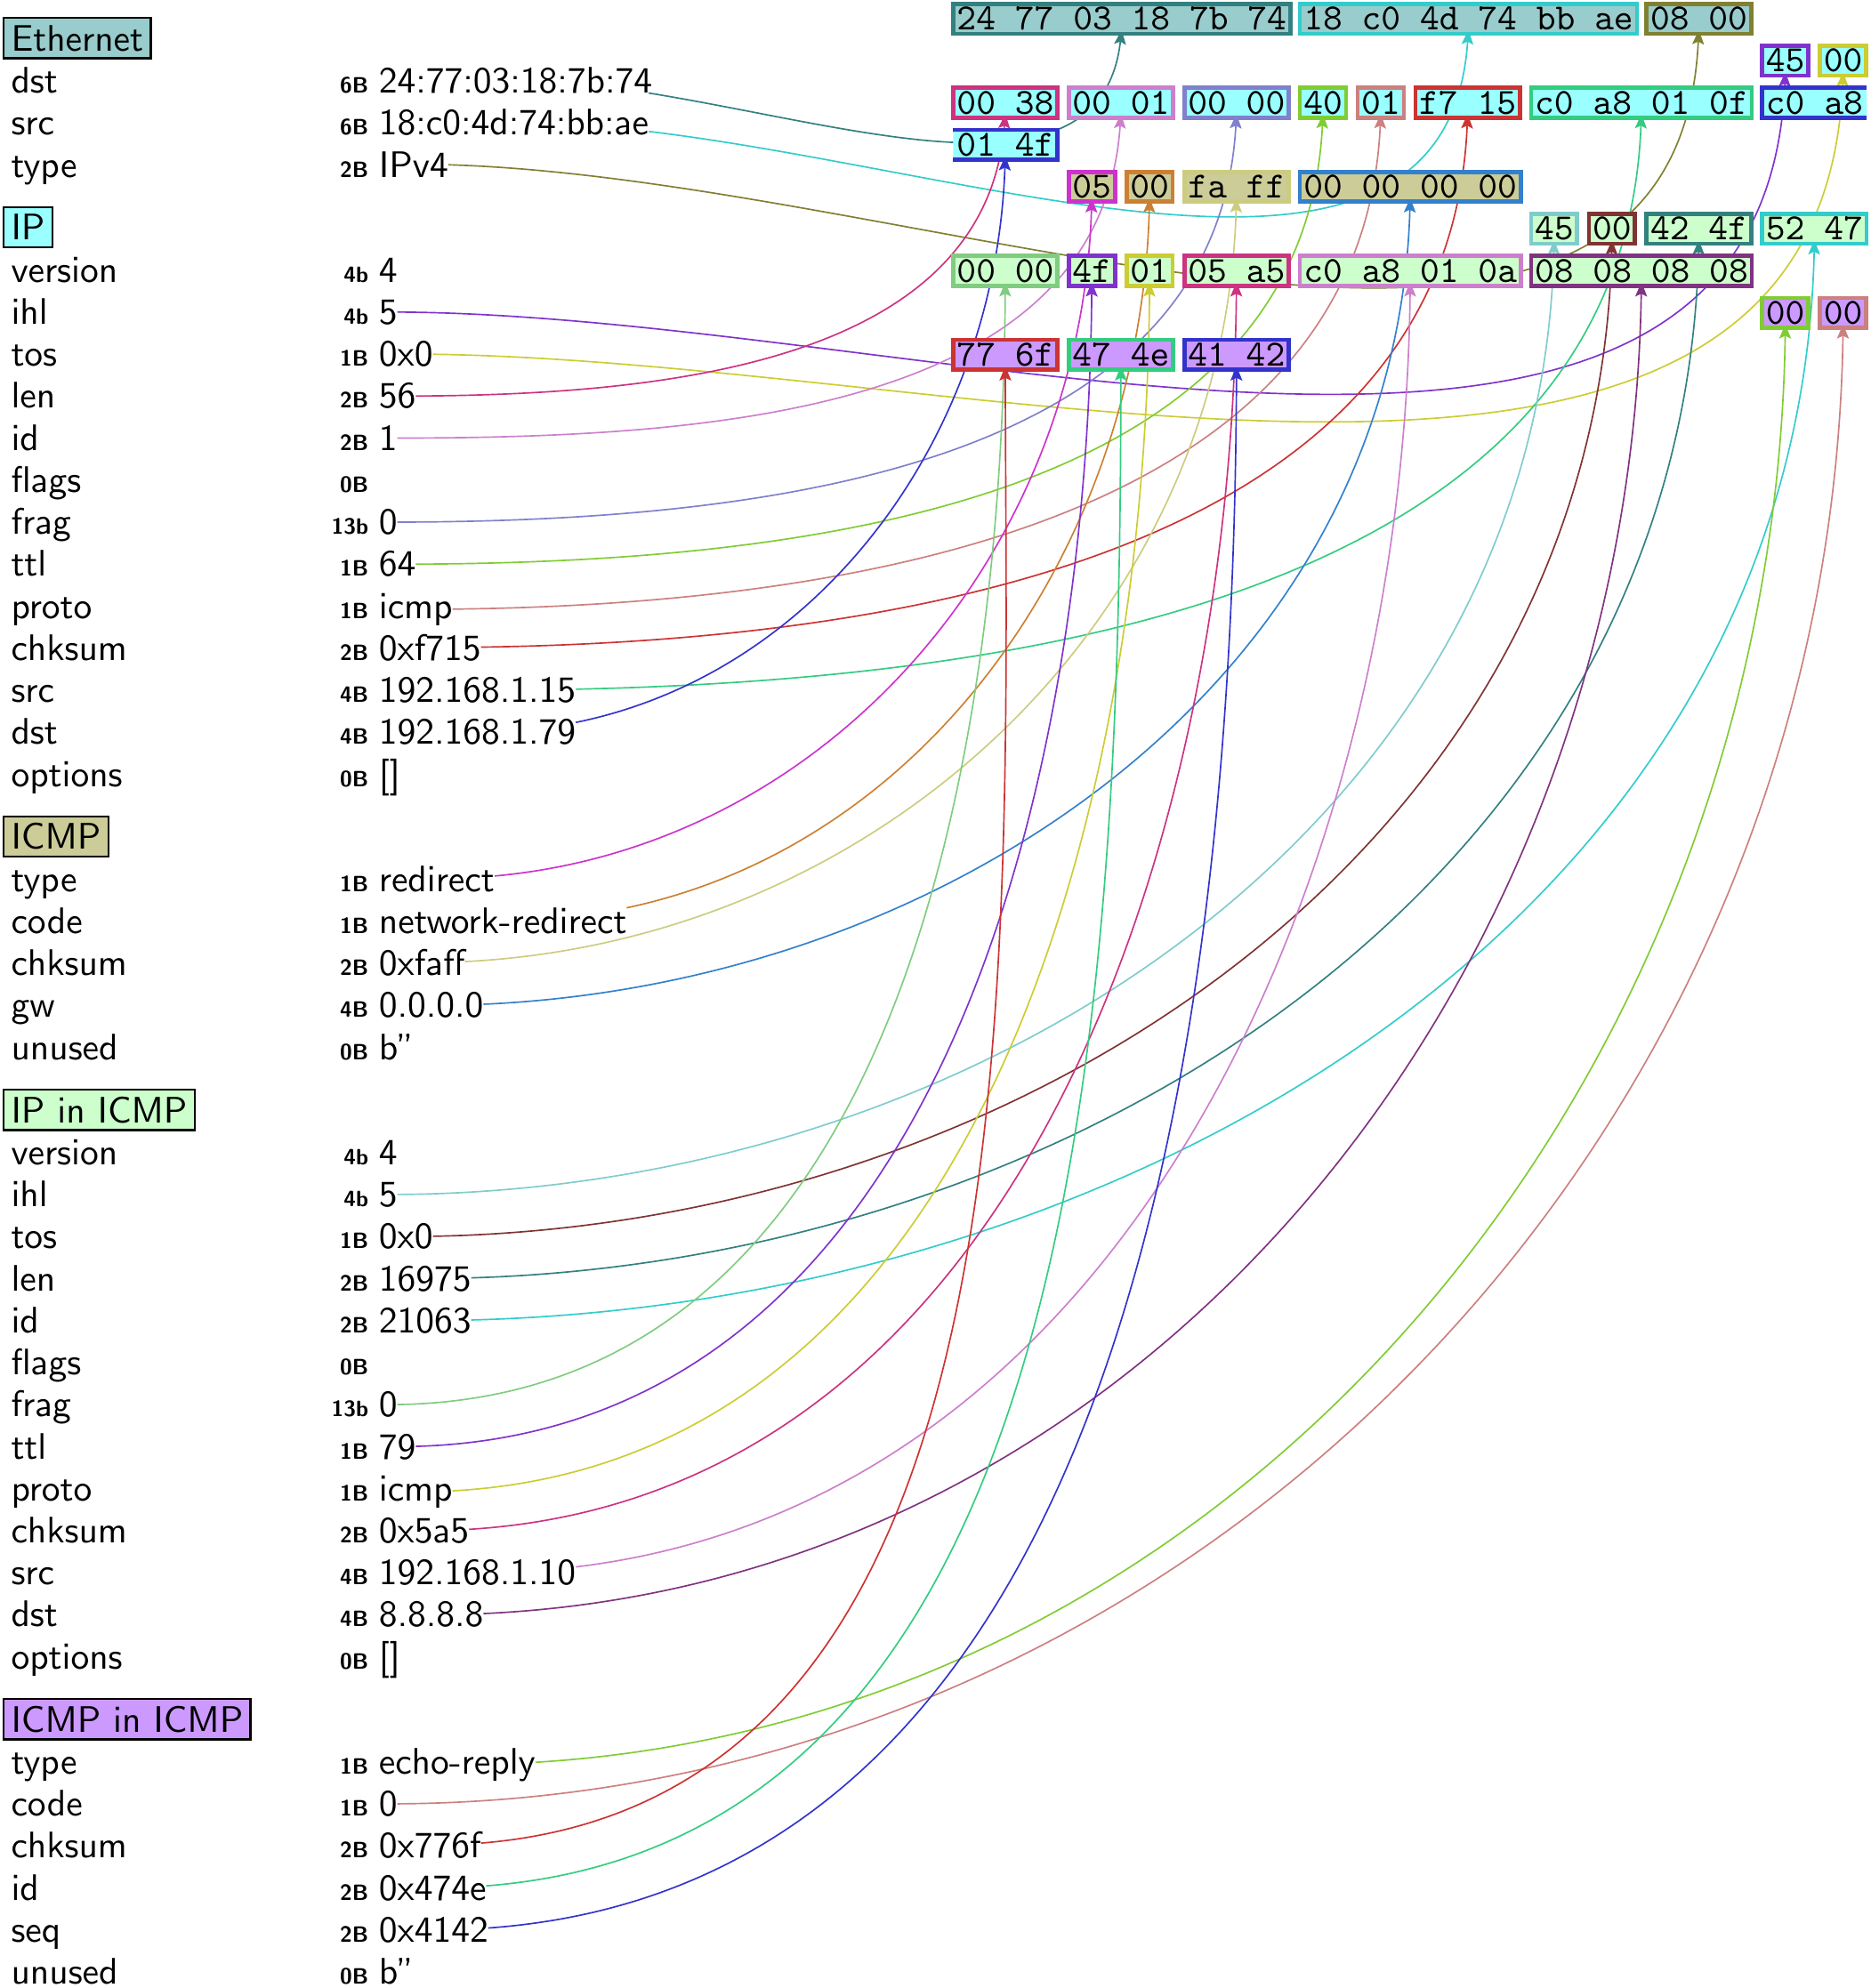
\includegraphics[width=0.6\textwidth]{../Tesi/img/pcap/packet_redirect_page_1.png}
%\captionof{figure}{Messaggio ICMP Redirect}   
%%\end{figure} 
%\end{frame} 

\begin{frame} 
\frametitle{Inserimento dei dati nel campo Header+64 bits} 
\begin{columns}[T,onlytextwidth]
\column{0.48\textwidth}   
\justifying 
Nel campo sono presenti l'header IP più 8 byte per 
una lunghezza complessiva di 28 byte.
\vspace{1ex} \newline 
Nel nostro caso si inserirà un pacchetto ICMP/IP e 
siccome non rappresenta un datagram da inviare ma 
già spedito, si possono sfruttare un maggior numero 
di campi. 
\vspace{1ex} \newline 
In questo campo si potranno quindi inserire \textbf{9 byte} di dati. 
\column{0.48\textwidth} 
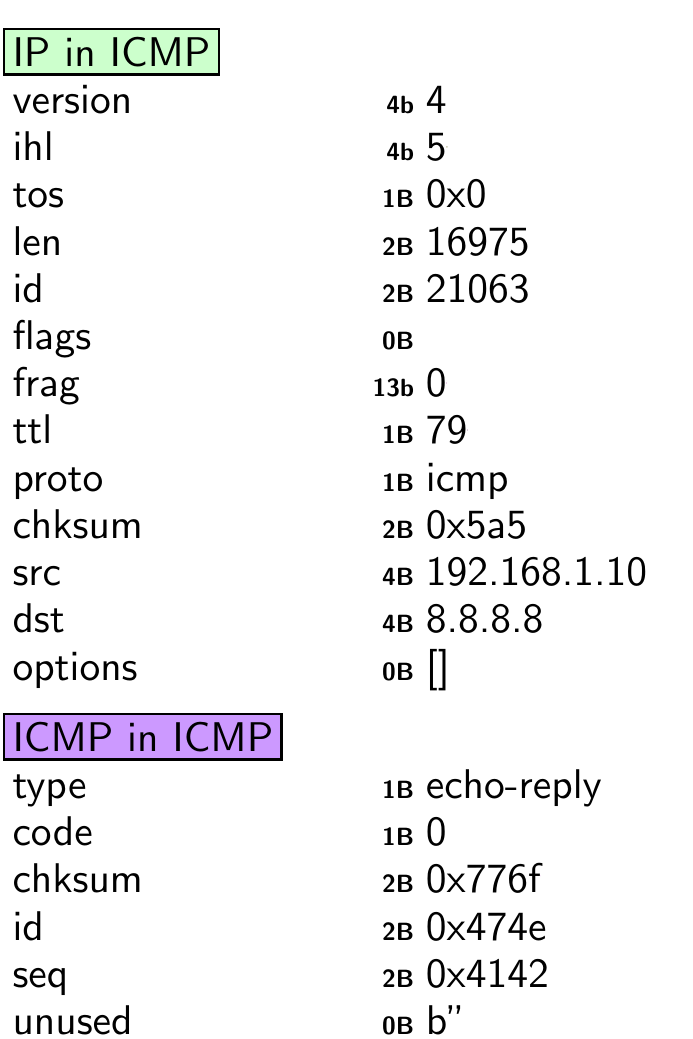
\includegraphics[width=0.7\textwidth]{../Tesi/img/ICMP_storageCC/immagie_header_64bit.png}
\captionof{figure}{Messaggio ICMP con campo \textit{Header+64 bit} impostato} 
\end{columns} 
\end{frame} 
\begin{frame} [fragile] 
\scriptsize
\begin{longtable}{|p{0.3\textwidth}|p{0.3\textwidth}|p{0.3\textwidth}|} 
    \multicolumn{3}{c}{Header IPv4} \\  
    \hline 
    \textbf{Campo} & \textbf{Byte} & \textbf{Utilizzo} \\
    \hline 
    Time to live & 1 byte & Tempo di vita del pacchetto\\  
    \hline 
    Total length & 2 byte & Dimensione dell'intero pacchetto\\  
    \hline
    Identification & 2 byte & Identifica i frammenti di un pacchetto IP \\ 
    \hline 
    \noalign{\vskip 2ex}
    \multicolumn{3}{c}{Header ICMPv4} \\ 
    \hline
    \textbf{Campo} & \textbf{Byte} & \textbf{Utilizzo} \\
    \hline
    %Aiuta nell'accoppiare le richieste e le risposte
    Identifier & 2 byte & Identificativo del messaggio di richiesta invocato \\  
    \hline 
    Sequence & 2 byte & Numero di sequenza del messaggio di richiesta invocato \\  
    \hline
    \caption{Uso del Header+64 bits nel caso di IP/ICMP} 
    \label{table:icmpv4:header64bit} 
\end{longtable}  
\end{frame}  
%\begin{frame}[fragile] %allowframebreaks
%\begin{lstlisting} [basicstyle=\ttfamily\scriptsize]
%0000  24 77 03 18 7B 74 18 C0 4D 74 BB AE 08 00 45 00  $w..{t..Mt....E.
%0010  00 38 00 01 00 00 40 01 F7 15 C0 A8 01 0F C0 A8  .8....@.........
%0020  01 4F 03 03 68 66 42 4F 52 47 45 00 4F 47 4E 41  .O..hfBORGE.OGNA
%0030  00 00 42 01 09 B3 C0 A8 01 0A 08 08 08 08 00 00  ..B.............
%0040  69 5E 4F 52 47 4F                                i^ORGO
%\end{lstlisting}
%\captionof{lstlisting}{Dump esadecimale del messaggio in figura precedente}
%\end{frame} 

%\begin{frame} [fragile]
%\frametitle{Destination Unreachable} 
%\footnotesize
%Sfrutta i campi \textbf{unused} e \textbf{header+64 bit}. Per una capacità 
%di esfiltrazione pari a \textbf{9+4 bytes}. \newline 
%\begin{center} 
%{\scriptsize 
%\begin{bytefield}[bitwidth=1.1em]{32} 
%	%\bitbox{8}{0} & \bitbox{8}{1} & \bitbox{8}{2} & \bitbox{8}{3} \\
%	\bitheader{0-31} \\
%	\bitbox{8}{Type=3 (1 byte)} & \bitbox{8}{Code=0-5 (1 byte)} & \bitbox{16}{Checksum (2 byte)} \\
%	\bitbox{32}{Unused (4 byte)} \\
%	\bitbox{32}{Internet Header + 64 bits of Original Datagram ($\geq$ 21 byte)} 
%\end{bytefield}  
%\captionof{figure}{Struttura del pacchetto \textbf{ICMPv4 Destination Unreachable}} 
%%Il campo \textit{Internet Header}: viene utilizzato dall'host per accoppiare il messaggio di errore al processo appropriato. 
%\vspace{1ex} 
%\begin{bytefield}[bitwidth=1.1em]{32} 
%	%\bitbox{8}{0} & \bitbox{8}{1} & \bitbox{8}{2} & \bitbox{8}{3} \\
%	\bitheader{0-31} \\
%	\bitbox{8} {Type=1 (1 byte)} & \bitbox{8}{Code=0-6 (1 byte)} & \bitbox{16}{Checksum (2 byte)} \\
%	\bitbox{32} {Unused (4 byte)} \\
%	\bitbox{32} {As much of invoking packet as possible without} \\
%	\bitbox{32} {the ICMPv6 packet exceeding the minimum IPv6 MTU ($\geq$ 0 byte)} 
%\end{bytefield} 
%\captionof{figure}{Struttura del pacchetto \textbf{ICMPv6 Destination Unreachable}} 
%%Il campo \textit{Invoking Packet} indica quanta parte del pacchetto (che ha attivato l'errore ICMPv6) debba essere inclusa. 
%%Il tutto senza eccedere il \textit{IPv6 MTU} il cui valore di default equivale a 1280 bytes.
%} \end{center} 
%\end{frame} 
%\begin{frame}
%%\begin{figure}
%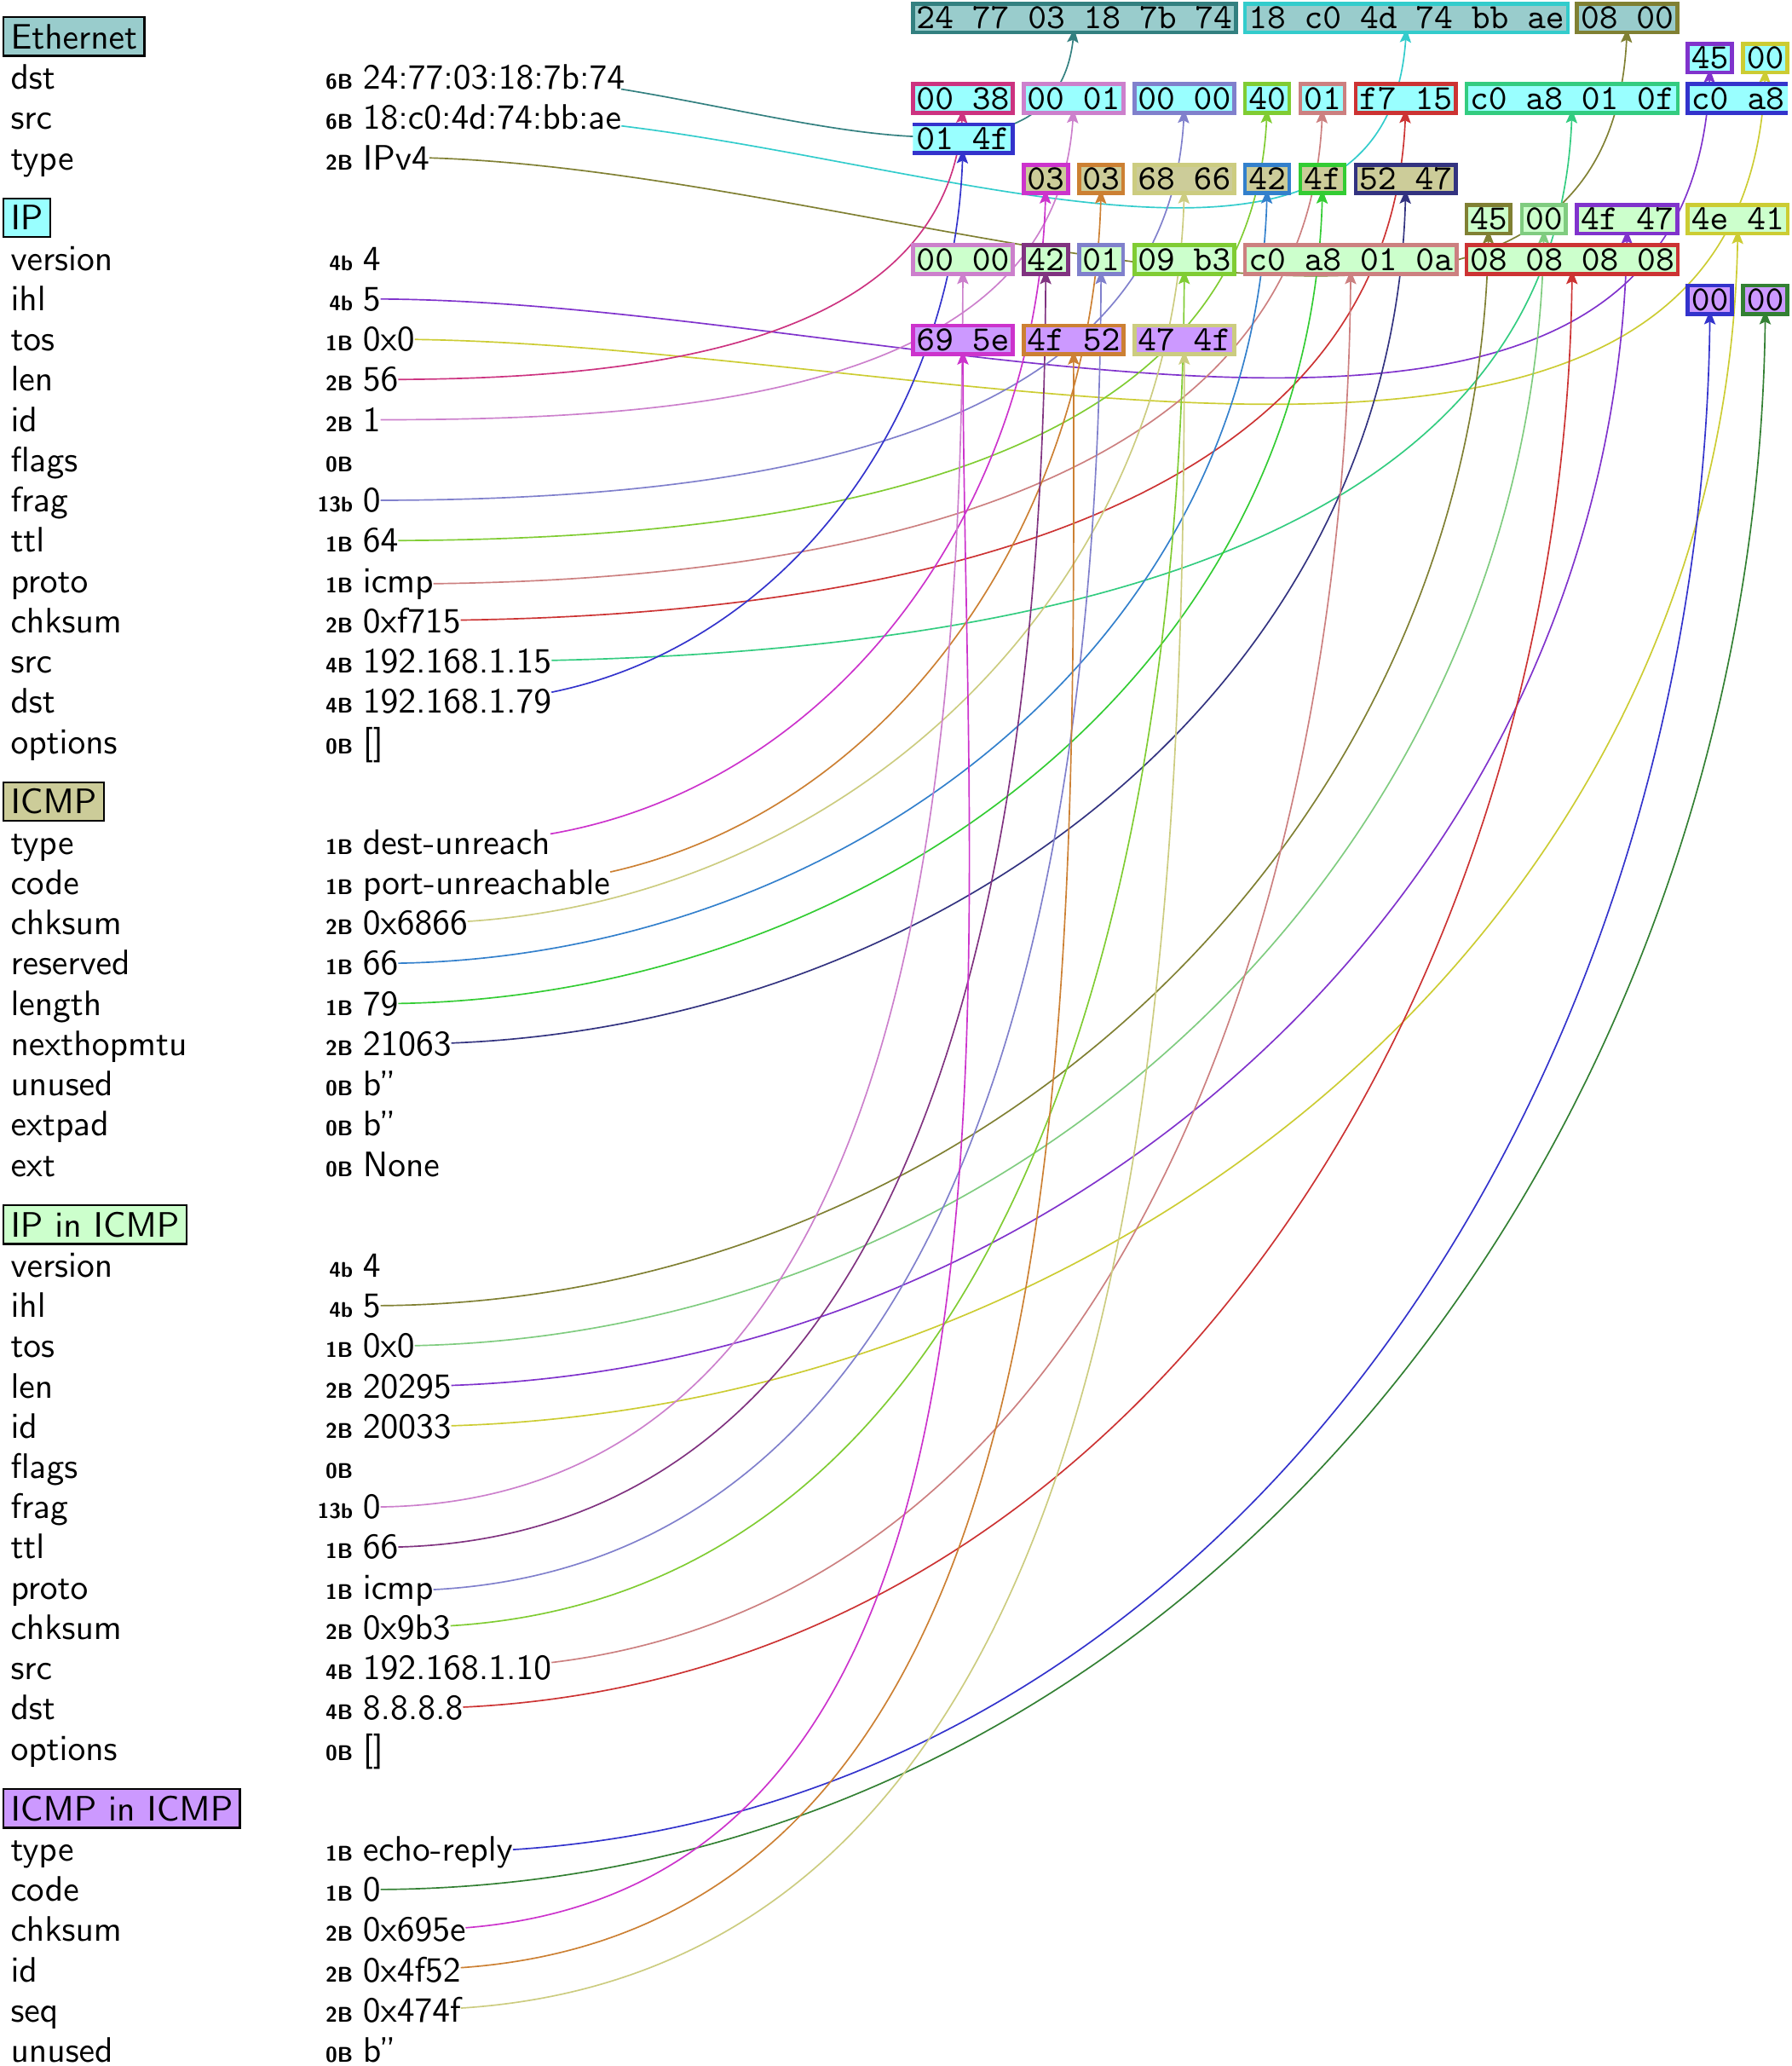
\includegraphics[width=0.6\textwidth]{../Tesi/img/pcap/packet_destination_unused_page_1.png}
%\captionof{figure}{Messaggio ICMP Destination Unreachable}   
%%\end{figure} 
%\end{frame} 

\begin{frame}
\frametitle{Inserimento dei dati nel campo Unused} 
\begin{columns}[T,onlytextwidth]
\column{0.48\textwidth}   
\justifying 
Dalle specifiche RFC (792 e 4434) il campo deve 
essere vuoto. 
Quindi utilizzando i metodi presenti nel 
framework Scapy per la creazione del paccheto, 
qualsiasi valore inserito al suo interno verrà azzerato. 
\vspace{1ex} \newline 
Il problema viene risolto tramite l'uso della 
libreria \textbf{struct}. Con essa è possibile 
costruire un pacchetto avente i dati all'interno del 
campo e successivamente si userà Scapy solo per l'invio. 
\column{0.48\textwidth} 
%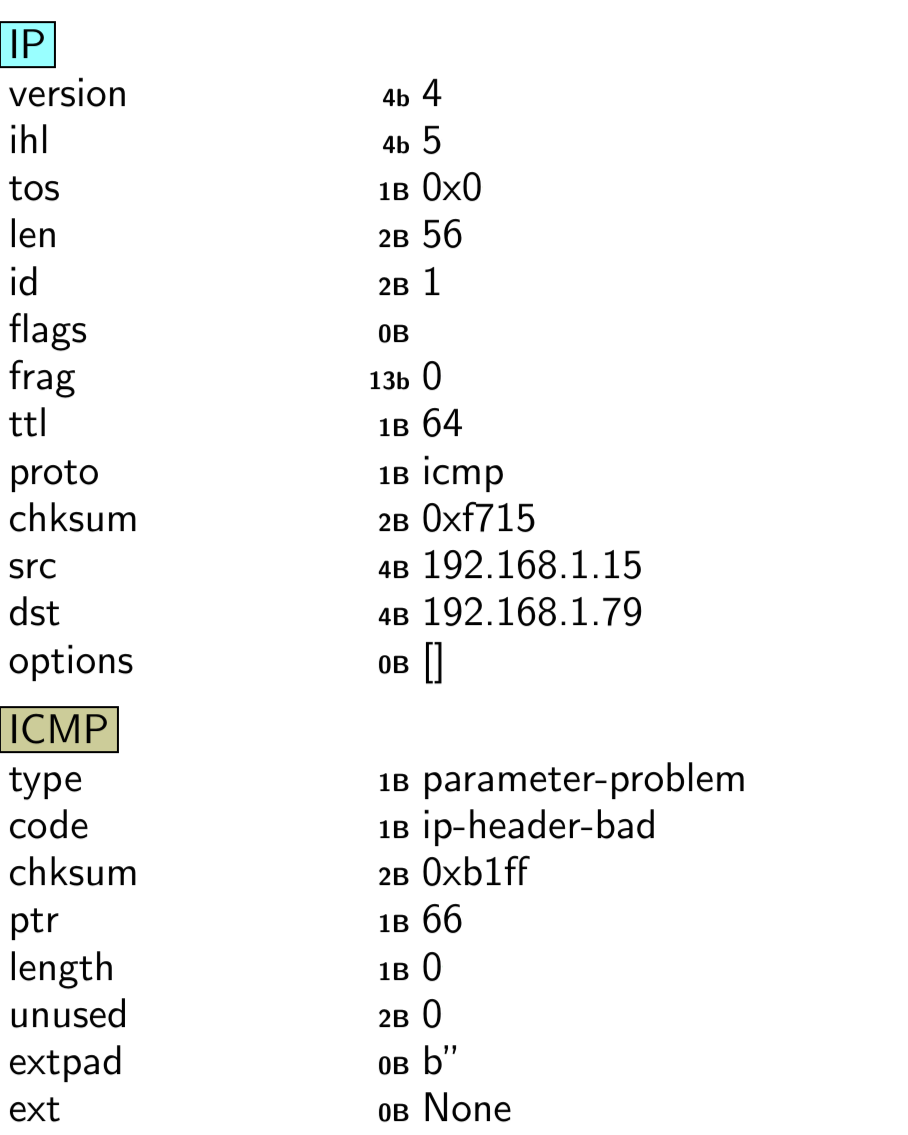
\includegraphics[width=0.8\textwidth]{../Tesi/img/ICMP_storageCC/immagine_parameterproblem.png}
%\captionof{figure}{Messaggio ICMP con campo \textit{unused} azzerato} 
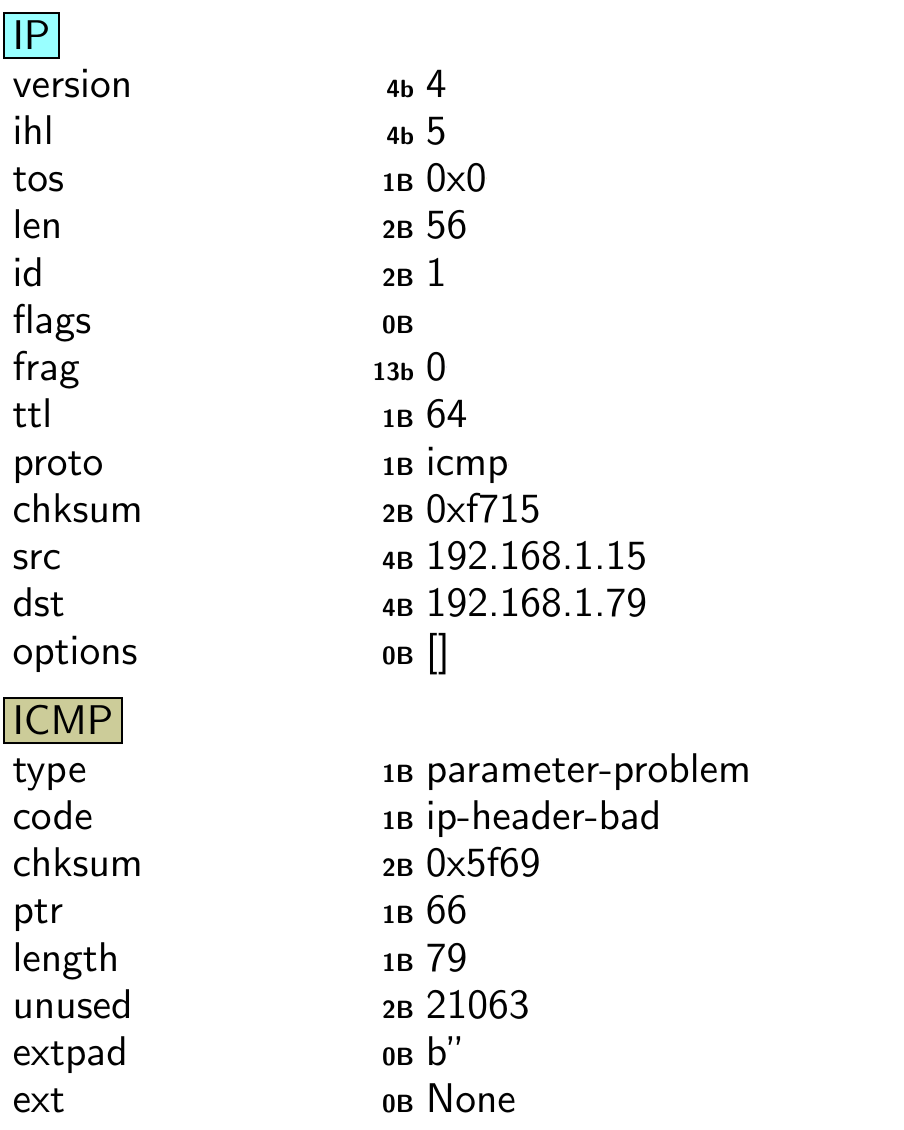
\includegraphics[width=0.9\textwidth]{../Tesi/img/ICMP_storageCC/immagine_parameterproblem_unused.png}
\captionof{figure}{Messaggio ICMP con campo \textit{unused} impostato}     
\end{columns} 
\end{frame}  

%\begin{frame} [fragile] 
%\frametitle{Time Exceeded} 
%\begin{center} 
%{\scriptsize 
%\begin{bytefield}[bitwidth=1.1em]{32} 
%        %\bitbox{8}{0} & \bitbox{8}{1} & \bitbox{8}{2} & \bitbox{8}{3} \\
%        \bitheader{0-31} \\
%        \bitbox{8}{Type=11 (1 byte)} & \bitbox{8}{Code=0-1 (1 byte)} & \bitbox{16}{Checksum (2 byte)} \\
%        \bitbox{32}{Unused (4 byte)} \\
%        \bitbox{32}{Internet Header + 64 bits of Original Datagram ($\geq$ 21 byte)} 
%\end{bytefield} 
%\captionof{figure}{Struttura del pacchetto \textbf{ICMPv4 Time Exceeded}}
%\vspace{1ex}  
%\begin{bytefield}[bitwidth=1.1em]{32} 
%        %\bitbox{8}{0} & \bitbox{8}{1} & \bitbox{8}{2} & \bitbox{8}{3} \\
%        \bitheader{0-31} \\
%        \bitbox{8} {Type=3 (1 byte)} & \bitbox{8}{Code=0-1 (1 byte)} & \bitbox{16}{Checksum (2 byte)} \\
%        \bitbox{32} {Unused (4 byte)} \\
%        \bitbox{32} {As much of invoking packet as possible without} \\
%        \bitbox{32} {the ICMPv6 packet exceeding the minimum IPv6 MTU ($\geq$ 0 byte)} 
%\end{bytefield}  
%\captionof{figure}{Struttura del pacchetto \textbf{ICMPv6 Time Exceeded}}
%} \end{center} 
%\end{frame} 
%\begin{frame}   
%\begin{figure}
%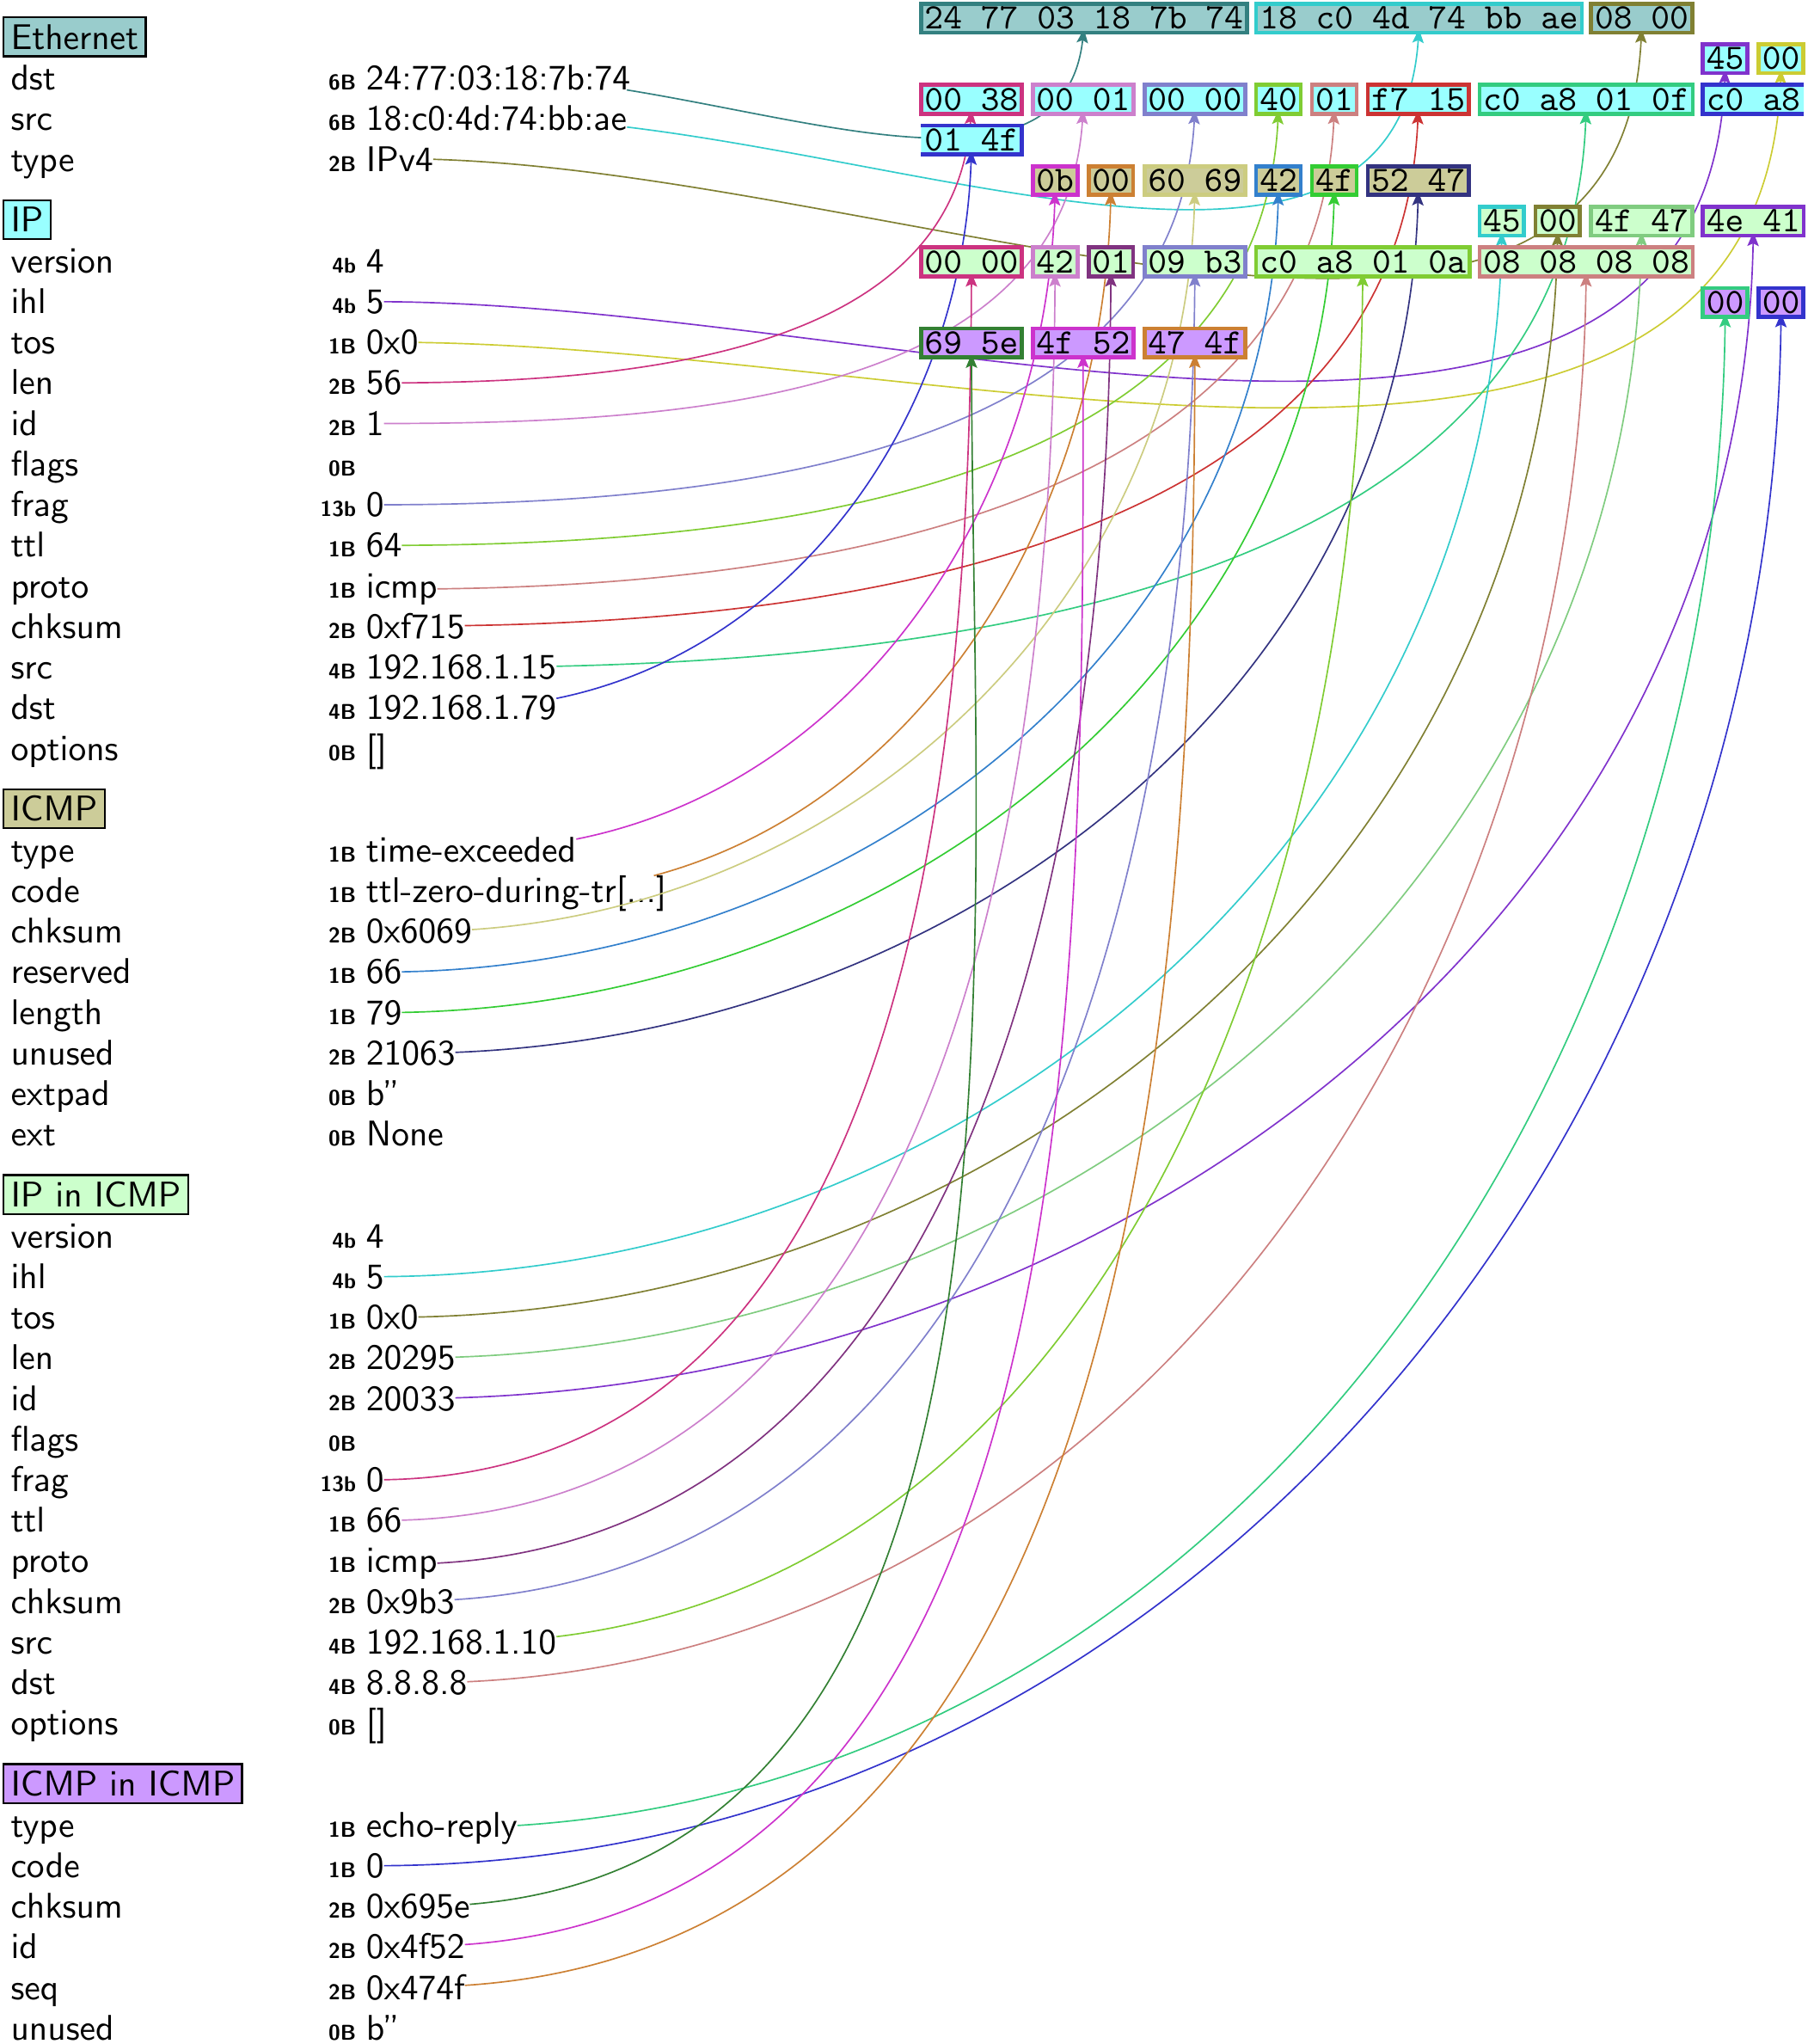
\includegraphics[width=0.6\textwidth]{../Tesi/img/pcap/packet_timeexceeded_unused_page_1.png}
%\captionof{figure}{Messaggio ICMP Time Exceeded}   
%\end{figure} 
%\end{frame} 

%\begin{frame} [fragile] 
%\frametitle{Source Quench}  
%\begin{center} 
%{\scriptsize 
%\begin{bytefield}[bitwidth=1.1em]{32} 
%        %\bitbox{8}{0} & \bitbox{8}{1} & \bitbox{8}{2} & \bitbox{8}{3} \\
%        \bitheader{0-31} \\
%        \bitbox{8}{Type=4 (1 byte)} & \bitbox{8}{Code=0 (1 byte)} & \bitbox{16}{Checksum (2 byte)} \\
%        \bitbox{32}{Unused (4 byte)} \\
%        \bitbox{32}{Internet Header + 64 bits of Original Datagram ($\geq$ 21 byte)} 
%\end{bytefield} 
%\captionof{figure}{Struttura del pacchetto \textbf{ICMPv4 Source Quench}} 
%} \end{center}  
%%\begin{figure}
%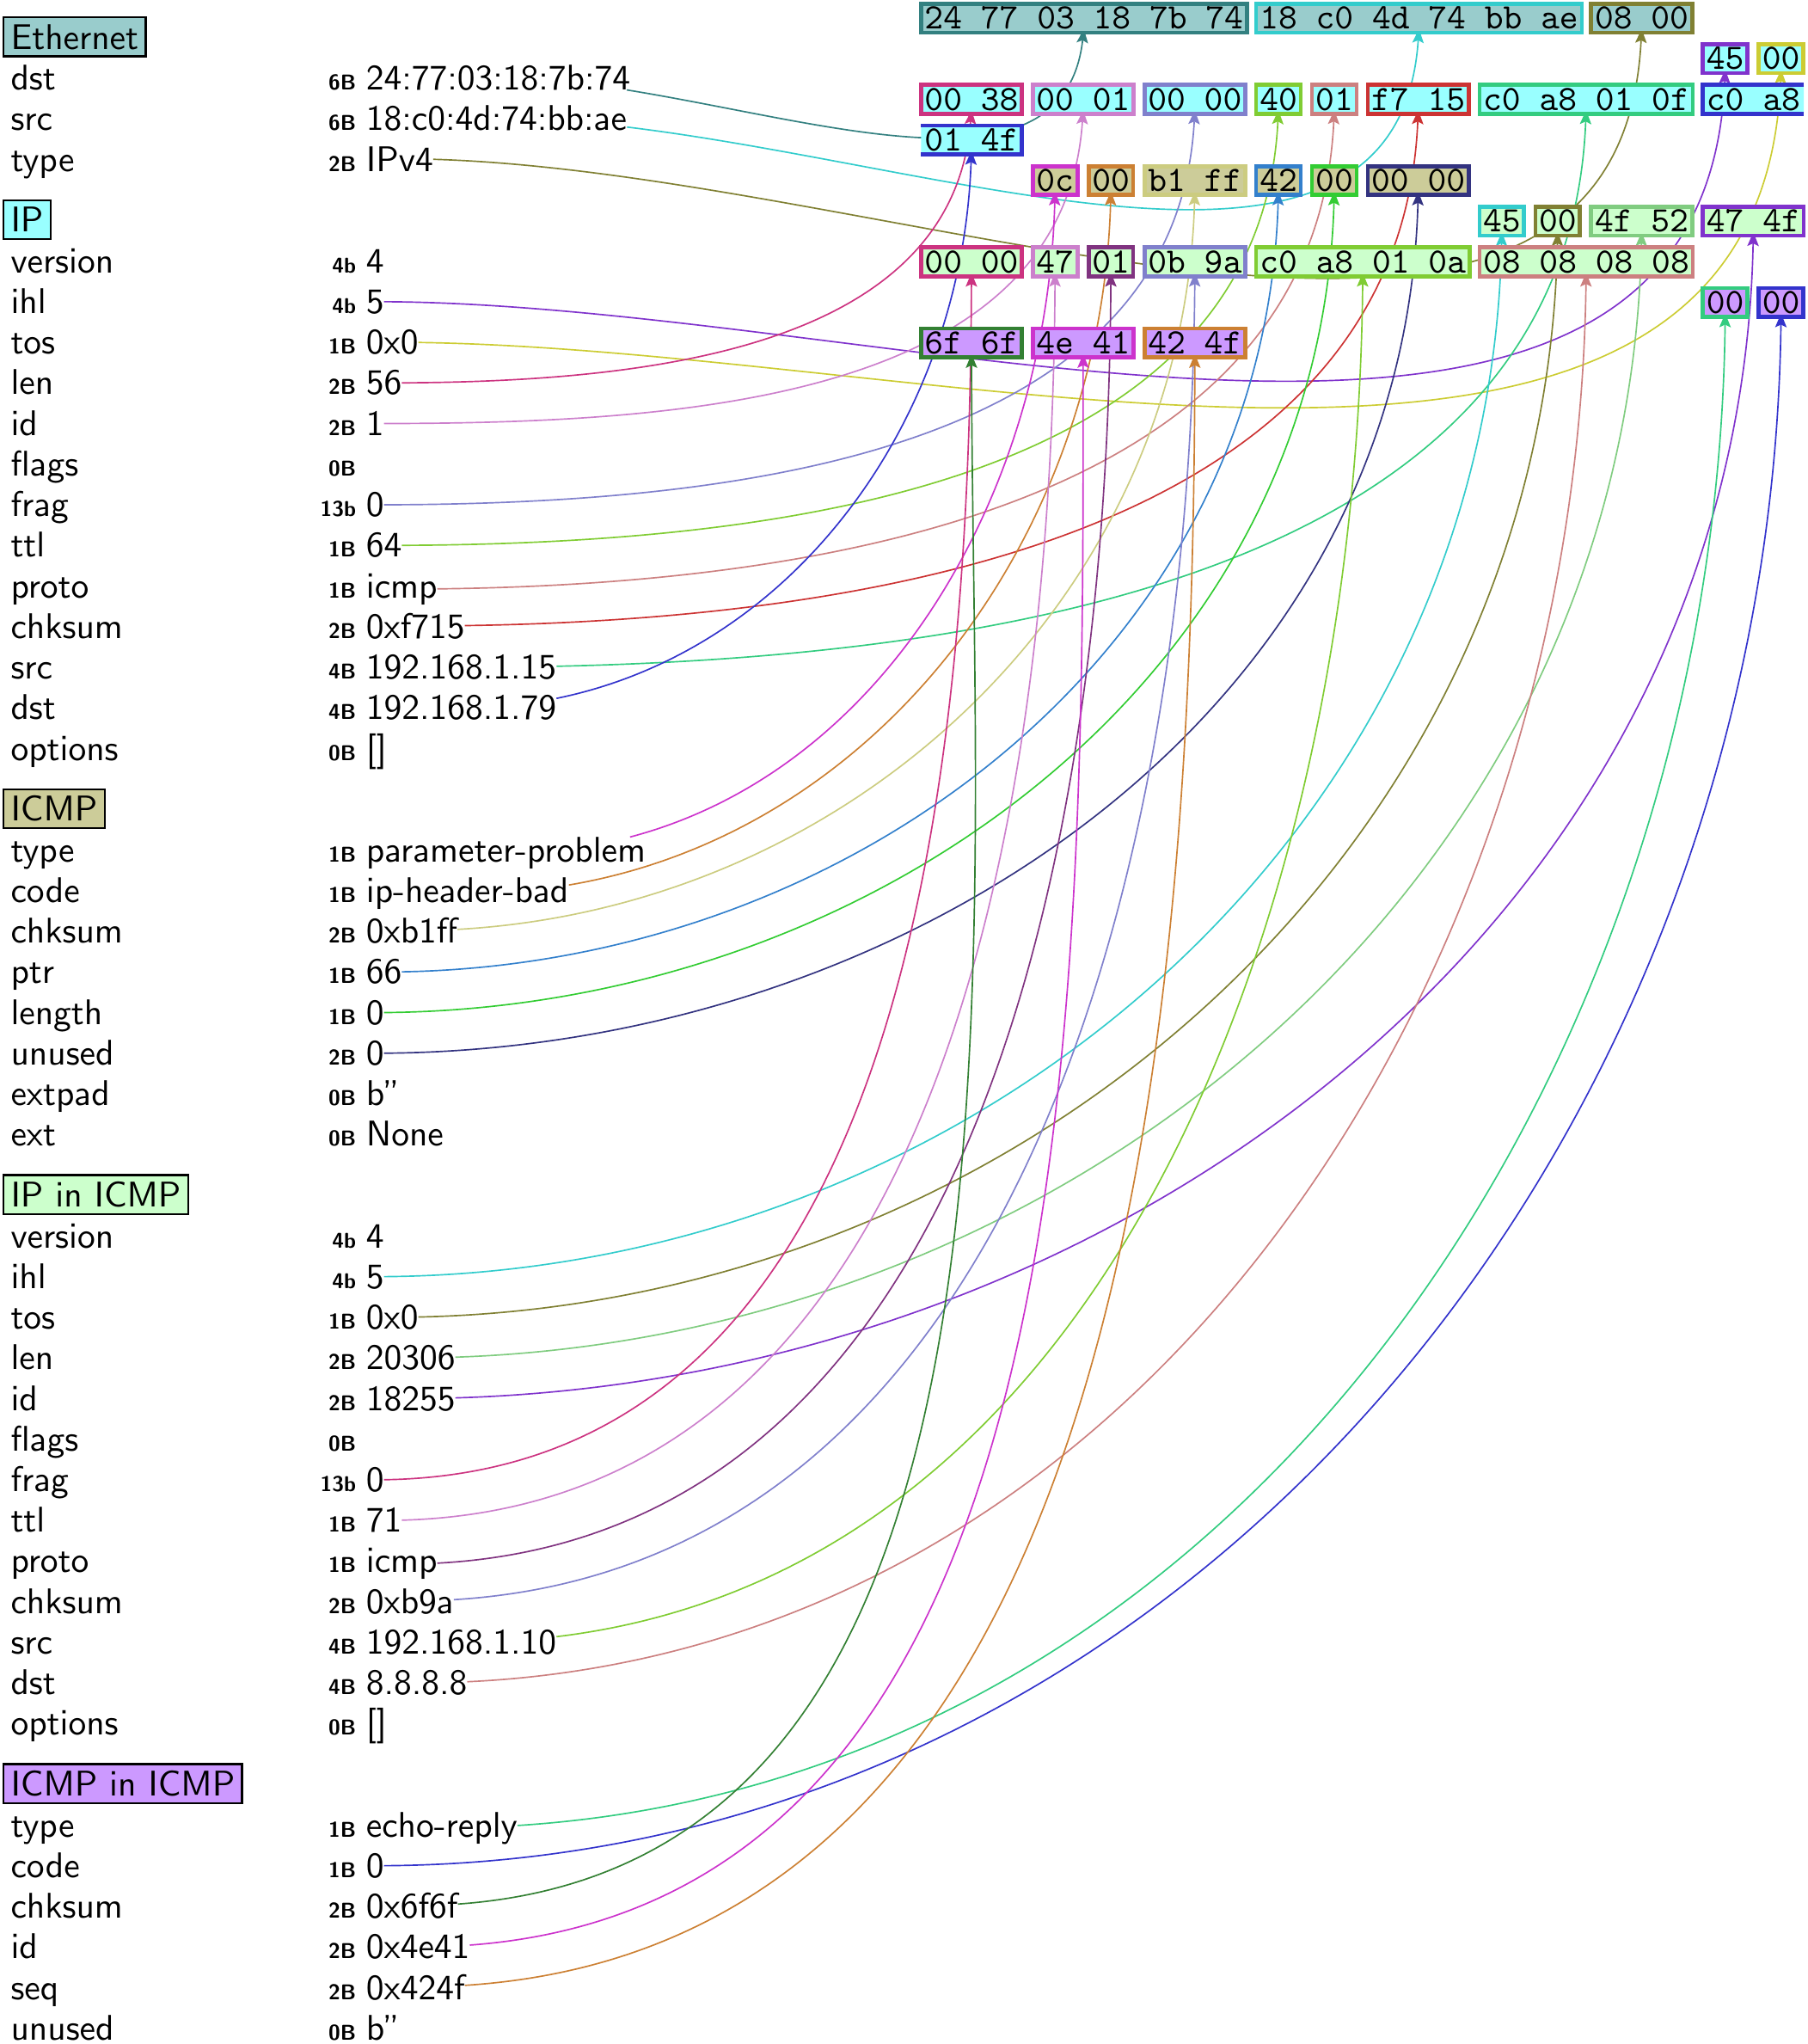
\includegraphics[width=0.3\textwidth]{../Tesi/img/pcap/packet_parameter_problem_page_1.png}
%\captionof{figure}{Messaggio ICMP source Quench}   
%%\end{figure} 
%\end{frame} 

%\begin{frame} [fragile] 
%\frametitle{Parameter Problem}  
%\begin{center} 
%{\scriptsize 
%\begin{bytefield}[bitwidth=1.1em]{32} 
%        %\bitbox{8}{0} & \bitbox{8}{1} & \bitbox{8}{2} & \bitbox{8}{3} \\
%        \bitheader{0-31} \\
%        \bitbox{8}{Type=12 (1 byte)} & \bitbox{8}{Code=0 (1 byte)} & \bitbox{16}{Checksum (2 byte)} \\
%        \bitbox{8}{Pointer (1 byte)} & \bitbox{24}{Unused (3 byte)} \\
%        \bitbox{32}{Internet Header + 64 bits of Original Datagram ($\geq$ 21 byte)} 
%\end{bytefield}  
%\captionof{figure}{Struttura del pacchetto \textbf{ICMPv4 Parameter Problem}}
%\vspace{1ex} 
%\begin{bytefield}[bitwidth=1.1em]{32} 
%        \bitheader{0-31} \\
%        \bitbox{8} {Type=4 (1 byte)} & \bitbox{8}{Code=0-2 (1 byte)} & \bitbox{16}{Checksum (2 byte)} \\
%        \bitbox{32} {Pointer (4 byte)} \\
%        \bitbox{32} {As much of invoking packet as possible without} \\
%        \bitbox{32} {the ICMPv6 packet exceeding the minimum IPv6 MTU ($\geq$ 0 byte)} 
%\end{bytefield} 
%\captionof{figure}{Struttura del pacchetto \textbf{ICMPv6 Parameter Problem}}
%} \end{center} 
%\end{frame} 
%\begin{frame}
%%\begin{figure}
%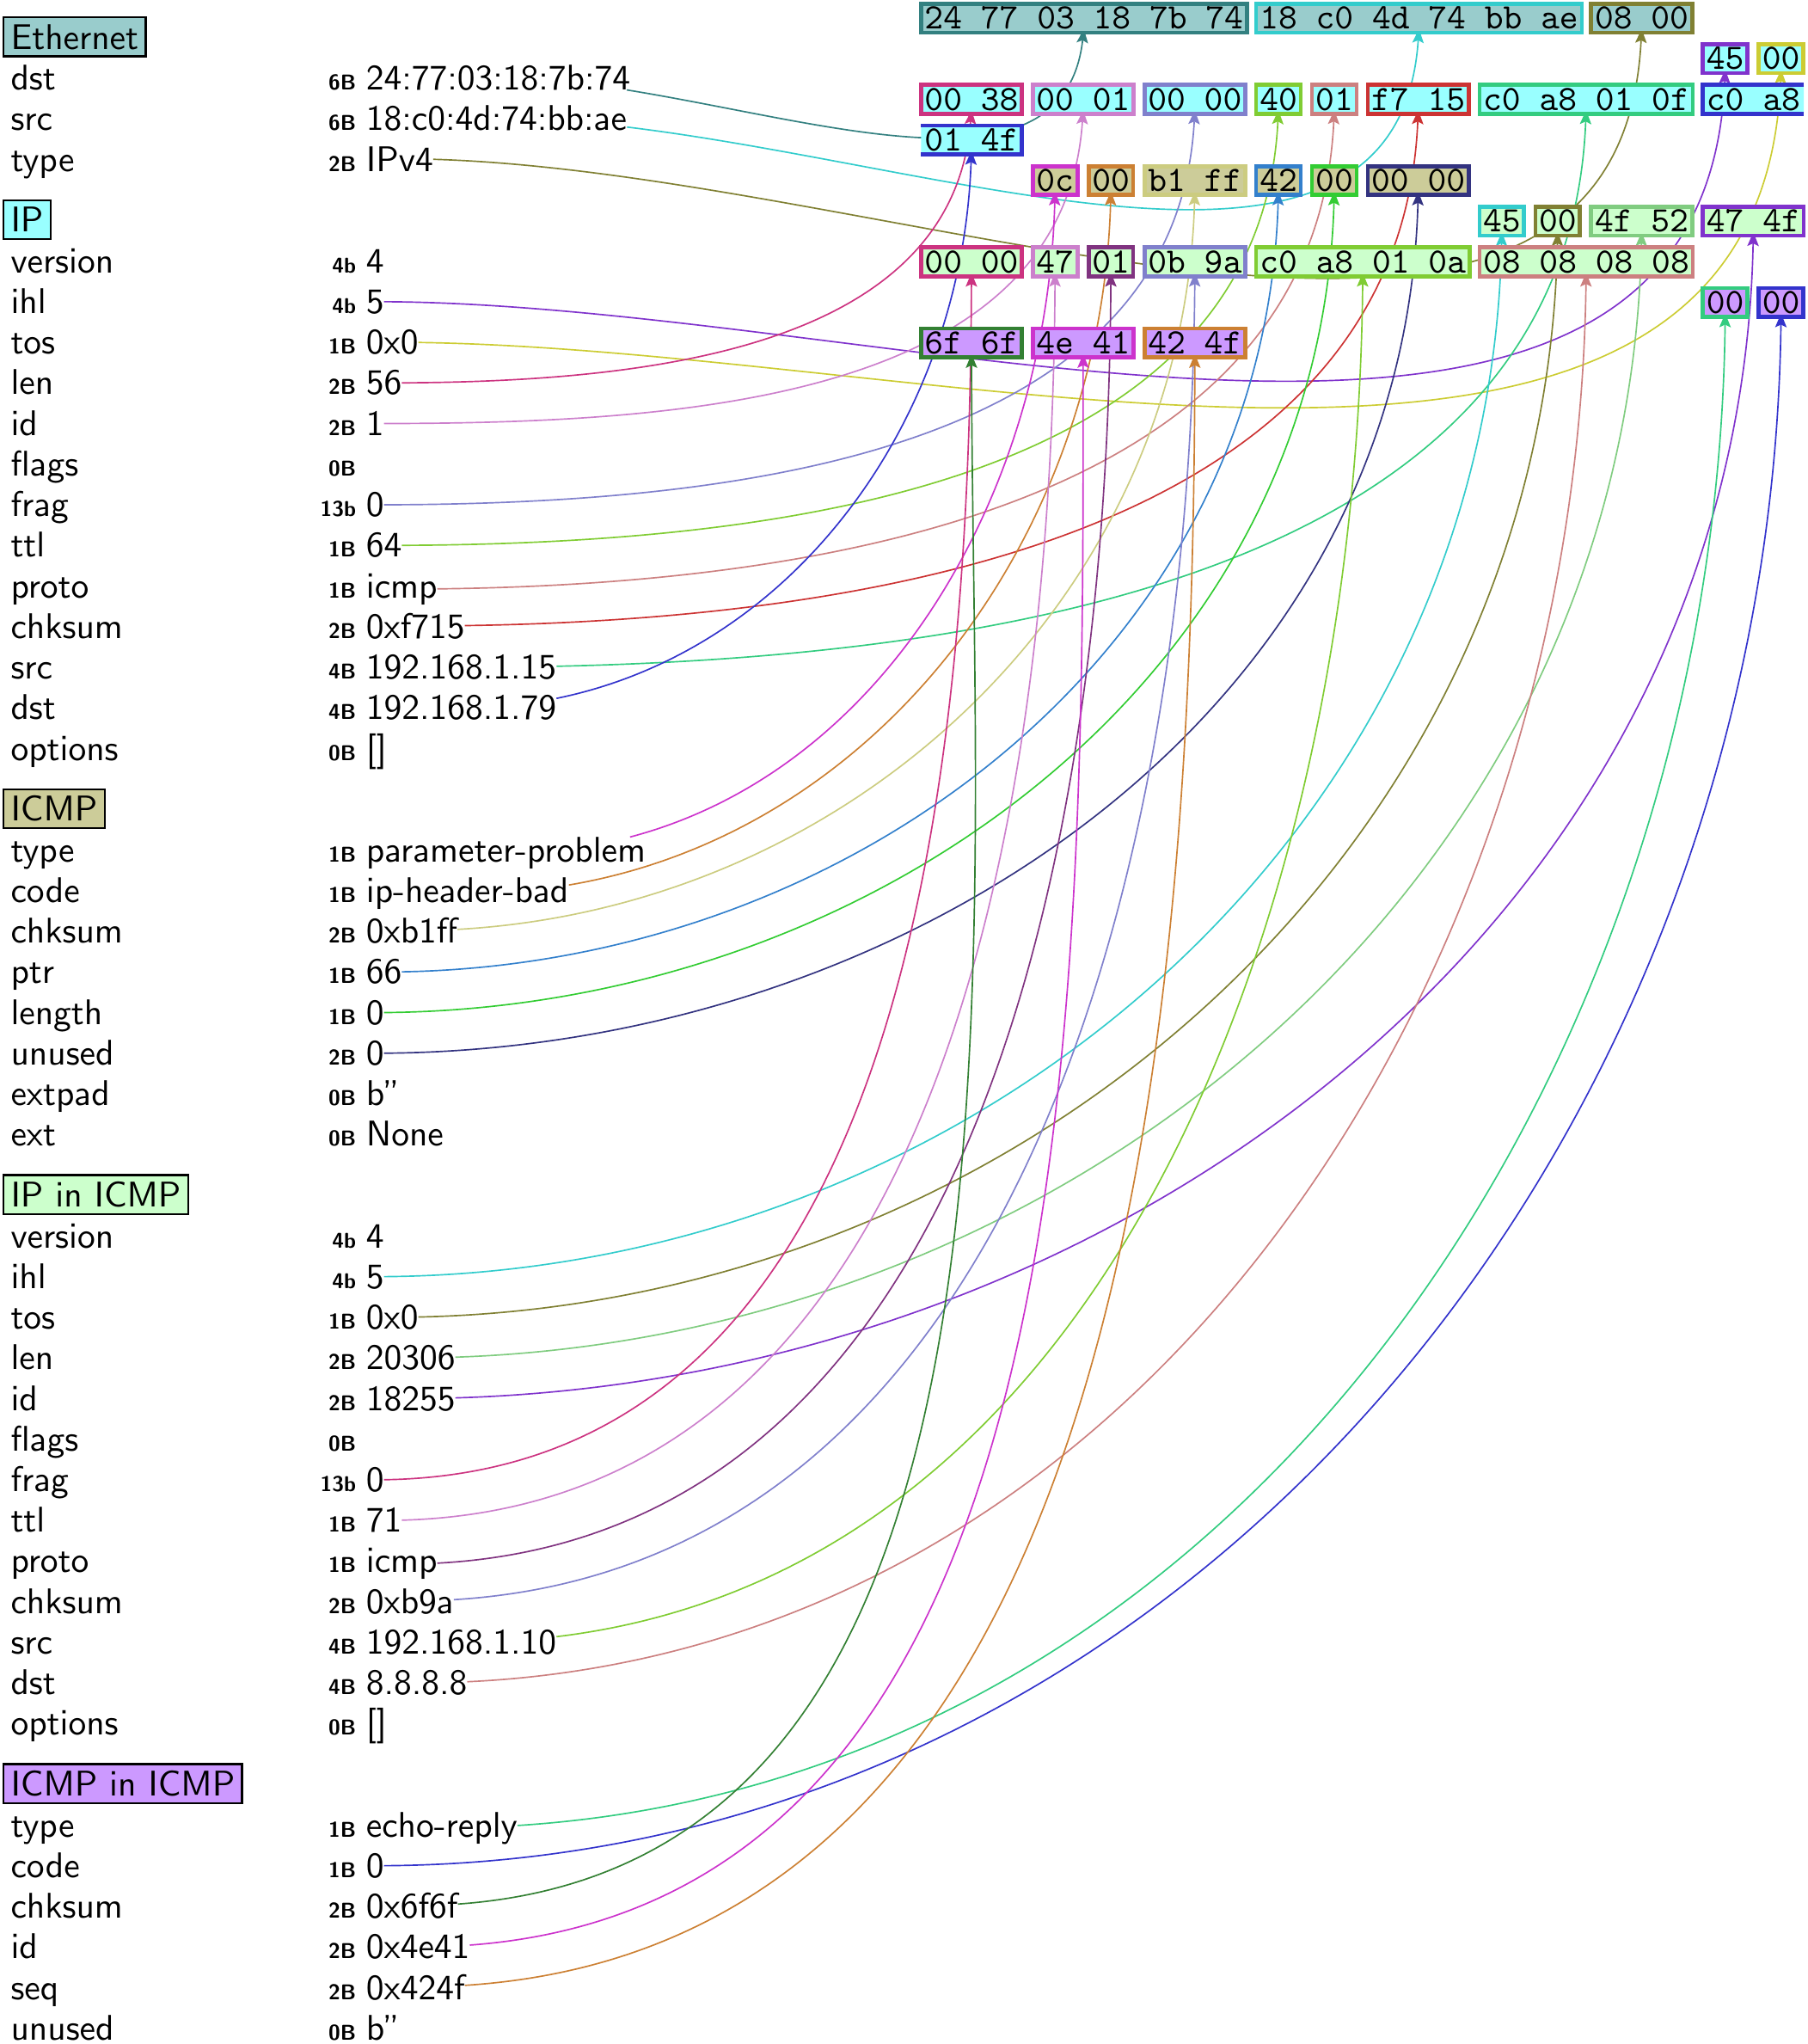
\includegraphics[width=0.6\textwidth]{../Tesi/img/pcap/packet_parameter_problem_page_1.png}
%\captionof{figure}{Messaggio ICMP Parameter Problem}   
%%\end{figure} 
%\end{frame} 

%\begin{frame} [fragile]
%\begin{lstlisting} [basicstyle=\ttfamily\scriptsize]
%0000  24 77 03 18 7B 74 18 C0 4D 74 BB AE 08 00 45 00  $w..{t..Mt....E.
%0010  00 38 00 01 00 00 40 01 F7 15 C0 A8 01 0F C0 A8  .8....@.........
%0020  01 4F 0C 00 B1 FF 42 00 00 00 45 00 4F 52 47 4F  .O....B...E.ORGO
%0030  00 00 47 01 0B 9A C0 A8 01 0A 08 08 08 08 00 00  ..G.............
%0040  6F 6F 4E 41 42 4F                                ooNABO
%\end{lstlisting}
%\captionof{lstlisting}{Dump esadecimale del messaggio in Figura \ref{fig:covertStorage:pointer}} 
%\end{frame} 

%\begin{frame} [fragile] 
%\frametitle{Information Request /Information Reply}  
%\begin{center} 
%{\scriptsize 
%\begin{bytefield}[bitwidth=1.1em]{32} 
%        %\bitbox{8}{0} & \bitbox{8}{1} & \bitbox{8}{2} & \bitbox{8}{3} \\
%        \bitheader{0-31} \\
%        \bitbox{8}{Type=15 (1 byte)} & \bitbox{8}{Code=0 (1 byte)} & \bitbox{16}{Checksum (2 byte)} \\
%        \bitbox{16}{Identifier (2 byte)} && \bitbox{16}{Sequence Number (2 byte)} 
%\end{bytefield} 
%\captionof{figure}{Struttura del pacchetto \textbf{ICMPv4 Information}} 
%} \end{center} 
%\begin{columns}[T,onlytextwidth]
%\column{0.48\textwidth}   
%\justifying 
%Il campo \textit{Identifier} definisce l'identificativo delle richieste e 
%può assumere un qualsiasi valore. Il campo \textit{Sequenza} (dalle 
%specifiche RFC 792), viene incrementato ad ogni richiesta inviata con lo 
%stesso identificativo. 
%\column{0.48\textwidth} 
%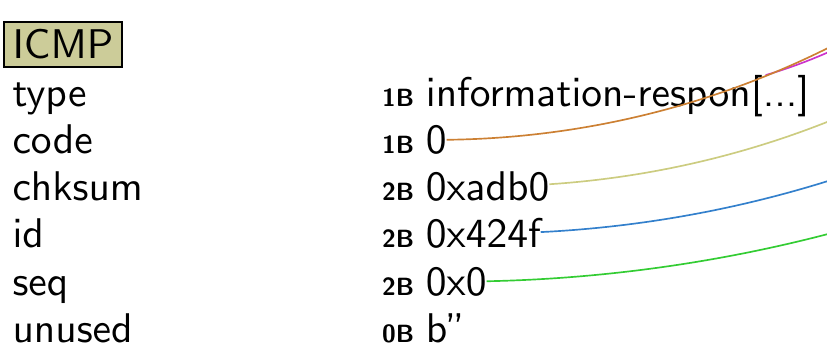
\includegraphics[width=\textwidth]{../Tesi/img/ICMP_storageCC/msgInformation_campoID.png}
%\captionof{figure}{Messaggio ICMP con campo \textit{identifier} impostato} 
%\end{columns}
%\end{frame} 
%\begin{frame} [fragile]
%\begin{lstlisting} [basicstyle=\ttfamily\scriptsize] 
%#PACCHETTO No1
%0000  24 77 03 18 7B 74 18 C0 4D 74 BB AE 08 00 45 00  $w..{t..Mt....E.
%0010  00 1C 00 01 00 00 40 01 F7 31 C0 A8 01 0F C0 A8  ......@..1......
%0020  01 4F 10 00 AD B0 42 4F 00 00                    .O....BO..
%
%#PACCHETTO No2
%0000  24 77 03 18 7B 74 18 C0 4D 74 BB AE 08 00 45 00  $w..{t..Mt....E.
%0010  00 1C 00 01 00 00 40 01 F7 31 C0 A8 01 0F C0 A8  ......@..1......
%0020  01 4F 10 00 9D B8 52 47 00 00                    .O....RG..
%
%#PACCHETTO No3
%0000  24 77 03 18 7B 74 18 C0 4D 74 BB AE 08 00 45 00  $w..{t..Mt....E.
%0010  00 1C 00 01 00 00 40 01 F7 31 C0 A8 01 0F C0 A8  ......@..1......
%0020  01 4F 10 00 A0 B8 4F 47 00 00                    .O....OG..
%
%#PACCHETTO No4
%0000  24 77 03 18 7B 74 18 C0 4D 74 BB AE 08 00 45 00  $w..{t..Mt....E.
%0010  00 1C 00 01 00 00 40 01 F7 31 C0 A8 01 0F C0 A8  ......@..1......
%0020  01 4F 10 00 A1 BE 4E 41 00 00                    .O....NA..
%\end{lstlisting}
%\captionof{lstlisting}{Dump esadecimale di quattro messaggi Information Request}
%\end{frame} 
%\begin{frame}
%%\begin{figure}
%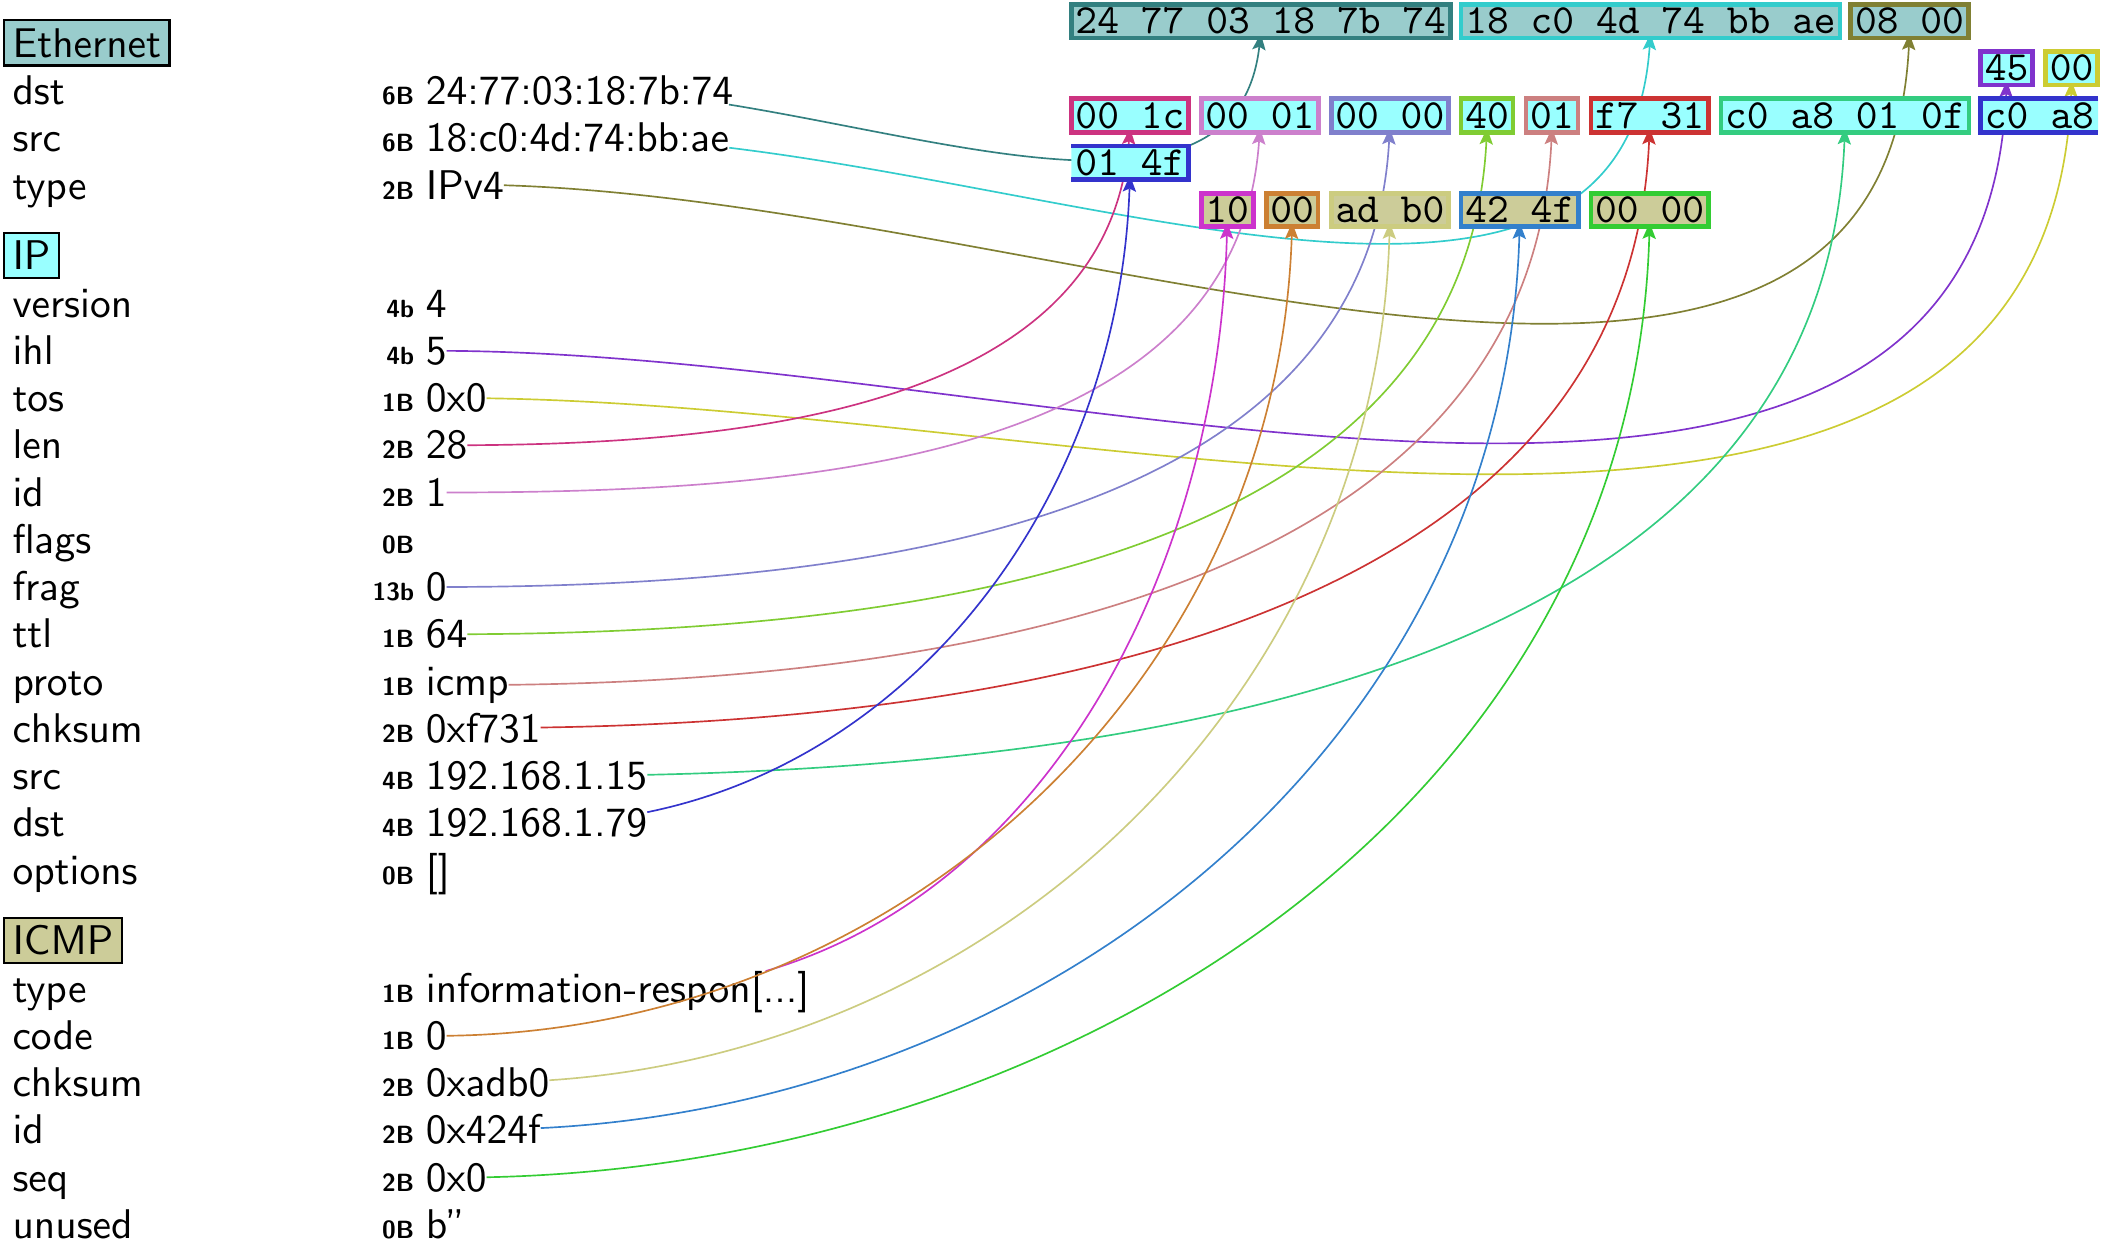
\includegraphics[width=\textwidth]{../Tesi/img/pcap/packet_information_1_page_1.png}
%\captionof{figure}{Messaggio ICMP Information Request/Reply}   
%%\end{figure} 
%\end{frame}   

%\begin{frame} [fragile] 
%\frametitle{Echo Request/Reply} 
%\begin{center} 
%{\scriptsize 
%\begin{bytefield}[bitwidth=1.1em]{32} 
%        %\bitbox{8}{0} & \bitbox{8}{1} & \bitbox{8}{2} & \bitbox{8}{3} \\
%        \bitheader{0-31} \\
%        \bitbox{8}{Type=8 (1 byte)} & \bitbox{8}{Code=0 (1 byte)} & \bitbox{16}{Checksum (2 byte)} \\
%        \bitbox{16}{Identifier (2 byte)} && \bitbox{16}{Sequence Number (2 byte)} \\
%        \bitbox{32}{Data ... ($\geq$ 0 byte)} 
%\end{bytefield}  
%\captionof{figure}{Struttura del pacchetto \textbf{ICMPv4 Echo}}
%\begin{bytefield}[bitwidth=1.1em]{32} 
%        %\bitbox{8}{0} & \bitbox{8}{1} & \bitbox{8}{2} & \bitbox{8}{3} \\
%        \bitheader{0-31} \\
%        \bitbox{8}{Type=128 (1 byte)} & \bitbox{8}{Code=0 (1 byte)} & \bitbox{16}{Checksum (2 byte)} \\
%        \bitbox{16}{Identifier (2 byte)} && \bitbox{16}{Sequence Number (2 byte)} \\
%        \bitbox{32}{Data ... ($\geq$ 0B)} 
%\end{bytefield} 
%\captionof{figure}{Struttura del pacchetto \textbf{ICMPv6 Echo}} 
%} \end{center} 
%\end{frame} 
%\begin{frame}
%%\begin{figure}
%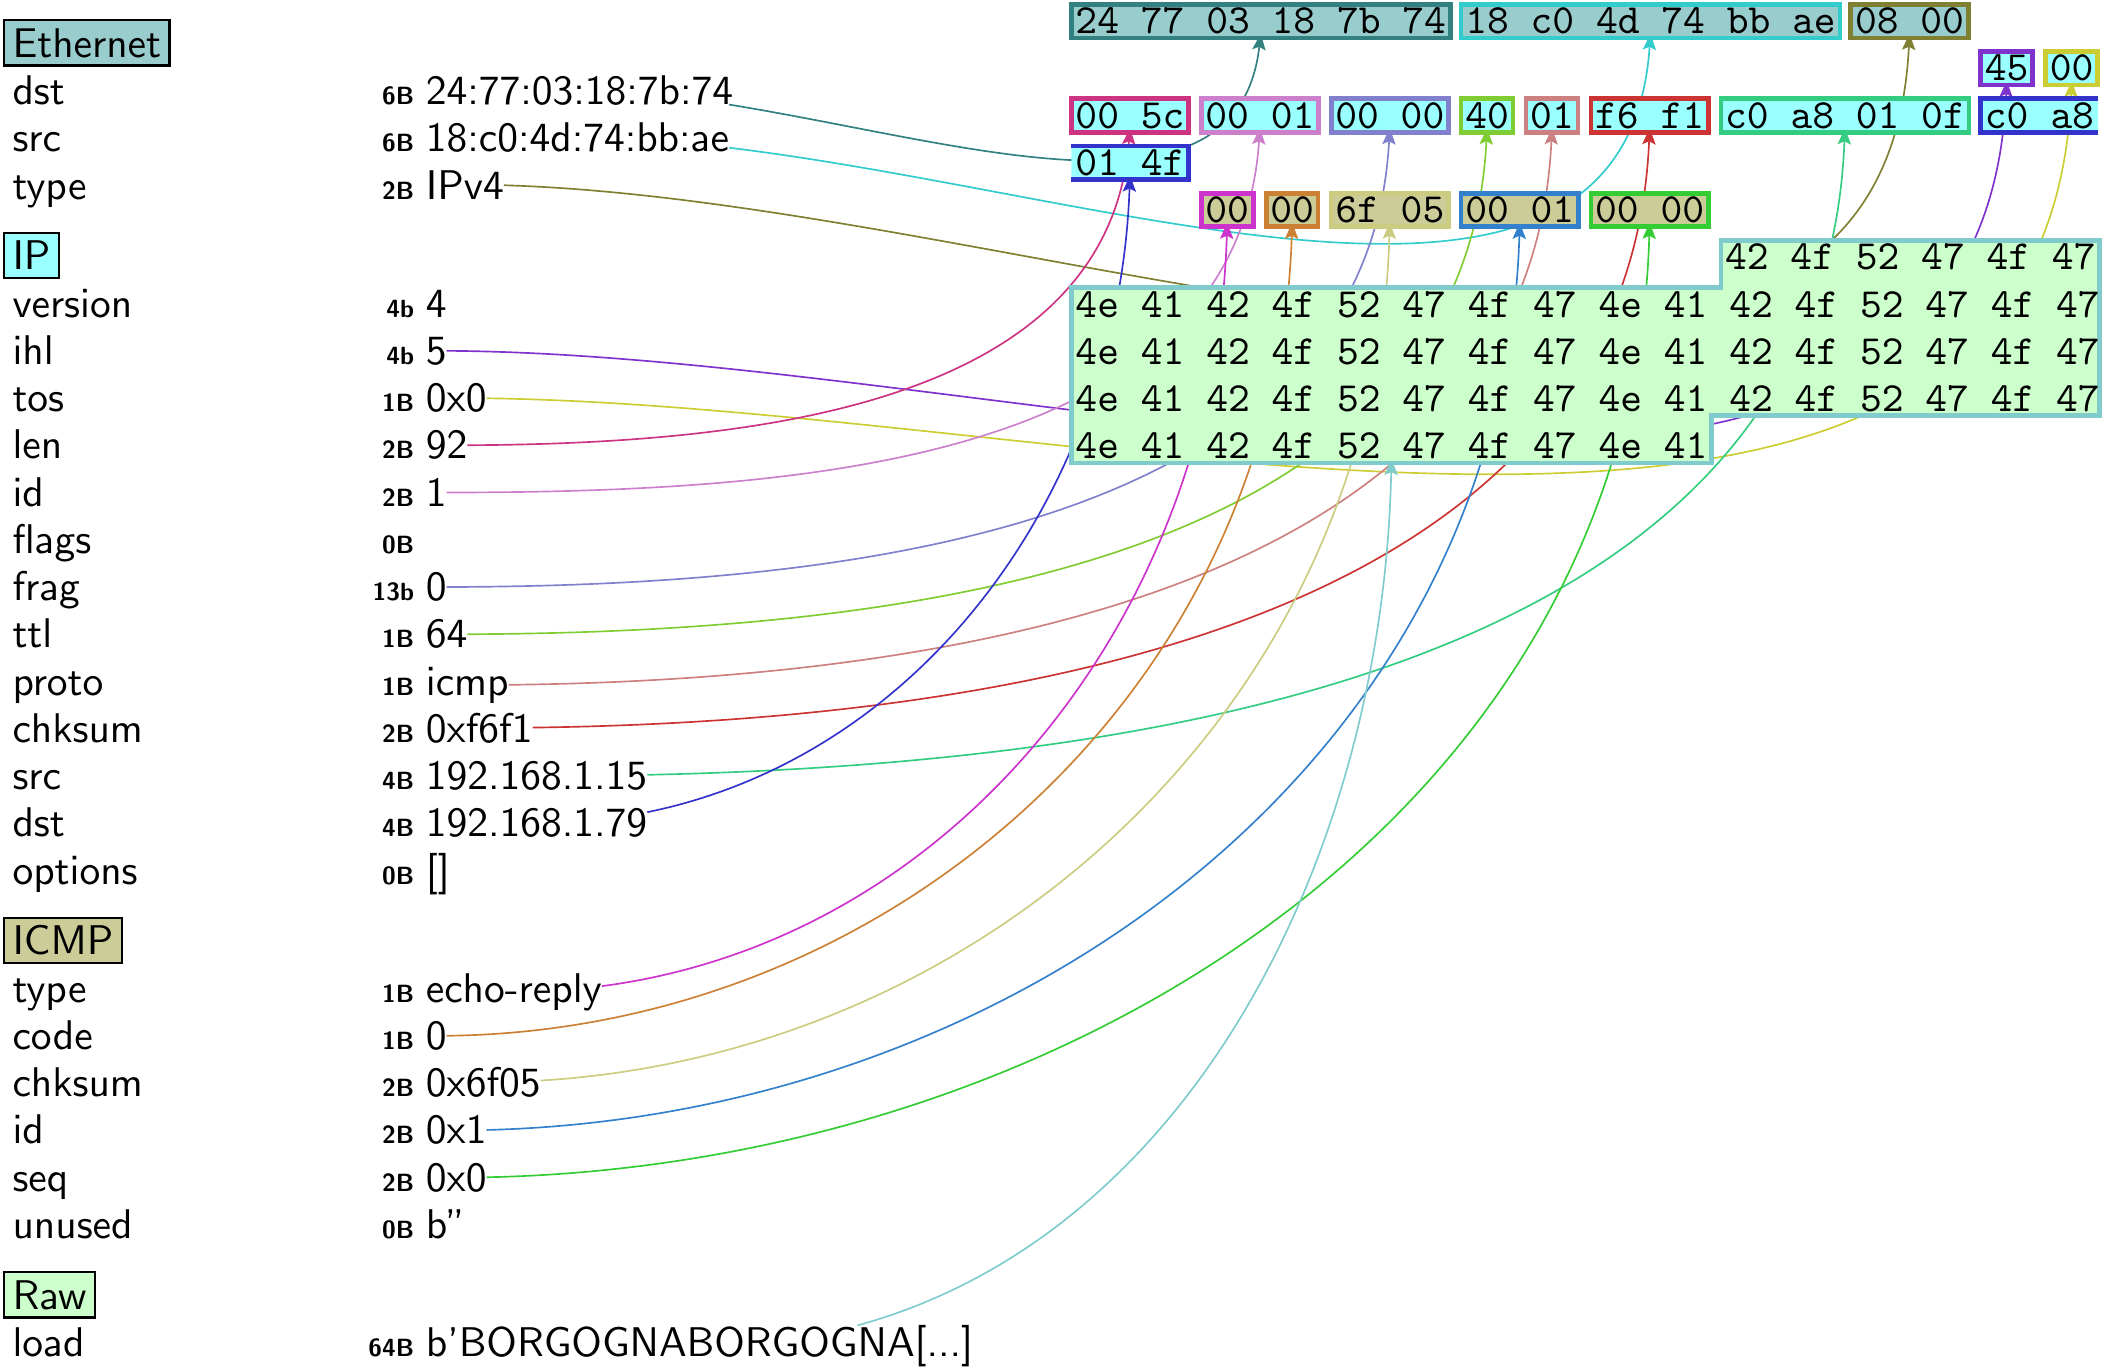
\includegraphics[width=\textwidth]{../Tesi/img/pcap/packet_echo_solo_payload_page_1.png}
%\captionof{figure}{Messaggio ICMP Echo Request/Reply}   
%%\end{figure} 
%\end{frame}  

\begin{frame} 
\frametitle{Inserimento dei dati nel campo Data} 
Nel campo il mittente può inserire quanti dati preferisce. Ma per sicurezza 
la dimensione sarà o 32 o 64 byte. Inoltre una quantità di dati eccessiva 
può far mandare più pacchetti di risposta nel caso si fosse inviata una richiesta. 
\begin{columns}[T,onlytextwidth]
\column{0.48\textwidth}   
\justifying 
%INSERIRE IMMAGINE IN CUOI SI MANDA NEL CMAPO DATA UN SACCO DI DATI TALE 
%CHE SI SAVRANNO TANTE REPLY
\column{0.48\textwidth} 
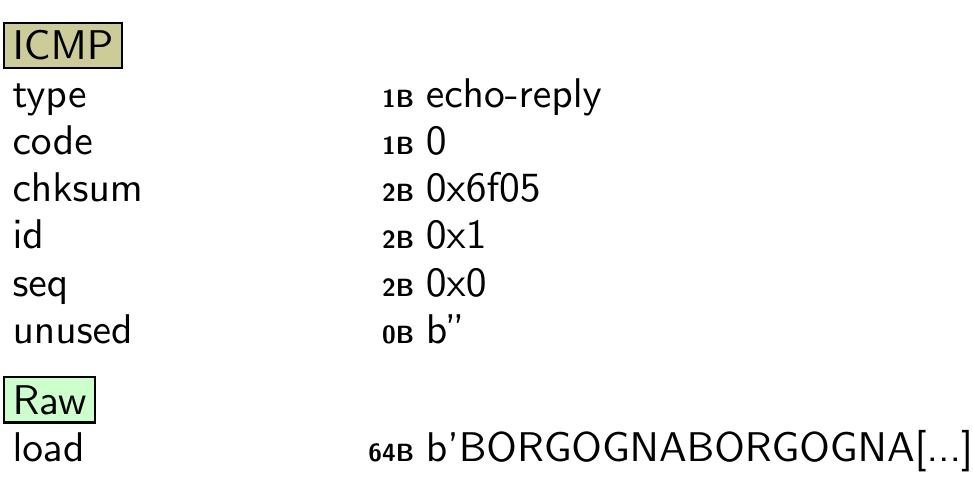
\includegraphics[width=\textwidth]{../Tesi/img/ICMP_storageCC/immagine_payload.png}
\captionof{figure}{Messaggio ICMP con campo \textit{Data} impostato} 
\end{columns}
\end{frame}  
%\begin{frame} [fragile] 
%\begin{lstlisting} [basicstyle=\ttfamily\scriptsize] 
%0000  24 77 03 18 7B 74 18 C0 4D 74 BB AE 08 00 45 00  $w..{t..Mt....E.
%0010  00 5C 00 01 00 00 40 01 F6 F1 C0 A8 01 0F C0 A8  .\....@.........
%0020  01 4F 00 00 6F 05 00 01 00 00 42 4F 52 47 4F 47  .O..o.....BORGOG
%0030  4E 41 42 4F 52 47 4F 47 4E 41 42 4F 52 47 4F 47  NABORGOGNABORGOG
%0040  4E 41 42 4F 52 47 4F 47 4E 41 42 4F 52 47 4F 47  NABORGOGNABORGOG
%0050  4E 41 42 4F 52 47 4F 47 4E 41 42 4F 52 47 4F 47  NABORGOGNABORGOG
%0060  4E 41 42 4F 52 47 4F 47 4E 41                    NABORGOGNA
%\end{lstlisting}
%\captionof{lstlisting}{Dump esadecimale del messaggio in Figura \ref{fig:covertStorage:payload}} 
%\end{frame} 

%\begin{frame} [fragile] 
%\frametitle{Timestamp Request/Reply}  
%\begin{center} 
%{\scriptsize 
%\begin{bytefield}[bitwidth=1.1em]{32} 
%        %\bitbox{8}{0} & \bitbox{8}{1} & \bitbox{8}{2} & \bitbox{8}{3} \\
%        \bitheader{0-31} \\
%        \bitbox{8}{Type=13 (1 byte)} & \bitbox{8}{Code=0 (1 byte)} & \bitbox{16}{Checksum (2 byte)} \\
%        \bitbox{16}{Identifier (2 byte)} && \bitbox{16}{Sequence Number (2 byte)} \\ 
%        \bitbox{32}{Originate Timestamp (4 byte)} \\
%        \bitbox{32}{Receive Timestamp (4 byte)} \\
%        \bitbox{32}{Transmit Timestamp (4 byte)} \\
%        \bitbox{32}{Data ... ($\geq$ 0 byte)} 
%\end{bytefield}
%\captionof{figure}{Struttura del pacchetto \textbf{ICMPv4 Timestamp}} 
%}\end{center} 
%Contiene i millisecondi dalla mezzanotte UT e ciascun campo ha un ordine 
%temporale specifico. Che dovrà rimanere congruente acnhe dopo che si sono 
%inseriti i dati.
%\end{frame} 
%\begin{frame}
%%\begin{figure}
%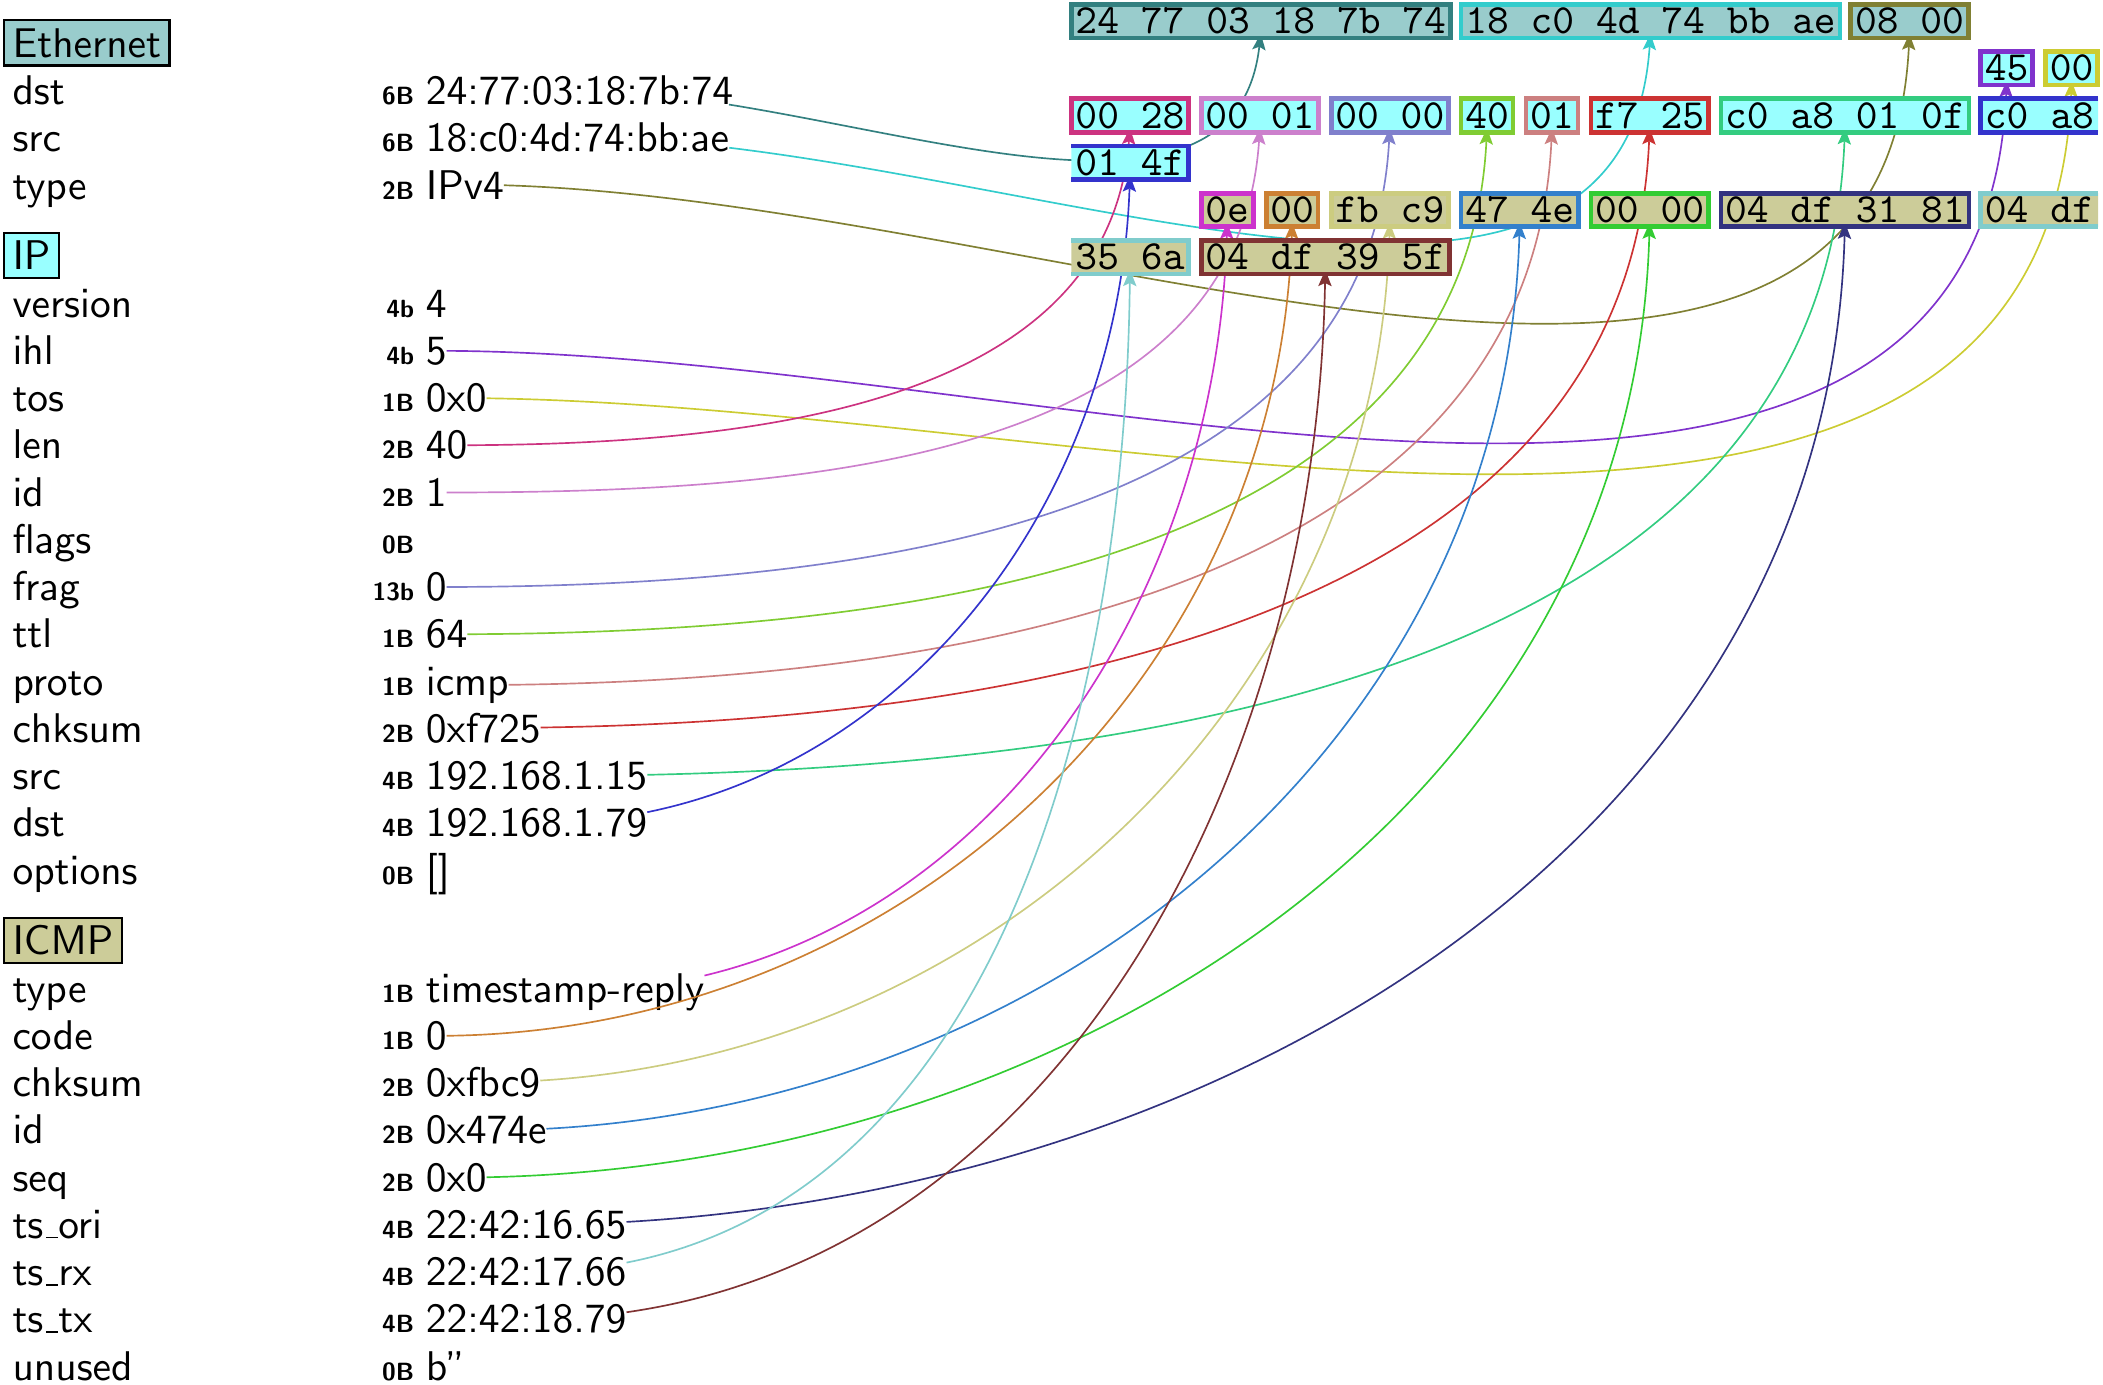
\includegraphics[width=\textwidth]{../Tesi/img/pcap/packet_timestamp_2_page_1.png}
%\captionof{figure}{Messaggio ICMP Timestamp Request/Reply}   
%%\end{figure} 
%\end{frame}  

\begin{frame} [fragile]
\frametitle{Inserimento dei dati nel campo Timestamp} 
\begin{columns}[T,onlytextwidth]
\column{0.48\textwidth}   
\justifying 
In ciascun campo timestamp verrà inserito un byte nella parte dei 
millisecondi. Non è possibile inserire ulteriori informazioni nelle altre 
parti  del campo siccome rappresentano le ore, i minuti ed i secondi. 
%Infatti hanno dei valori definiti e limitati, come si vede (che mostra il valore contenuto nei campi). 
Un alternativa è l'inserire il dato in tutto il campo ma, rappresentando 
un valore temporale, cio porterebbe al rischio di avere tempi errati o non 
congruenti. Per esempio il pacchetto risulta ricevuto prima che 
sia stato inviato. 
\column{0.48\textwidth} 
%\begin{figure}
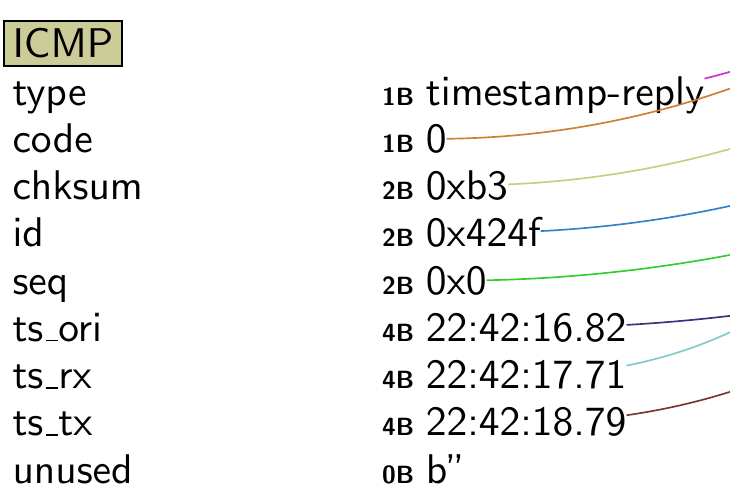
\includegraphics[width=\textwidth]{../Tesi/img/ICMP_storageCC/packet_timestamp_campo.png}
\captionof{figure}{Messaggio ICMP Timestamp Request/Reply}   
%\end{figure} 
\end{columns}
\end{frame}  
%\begin{frame} [fragile]
%\begin{lstlisting} [basicstyle=\ttfamily\scriptsize] 
%#PACCHETTO No1
%0000  24 77 03 18 7B 74 18 C0 4D 74 BB AE 08 00 45 00  $w..{t..Mt....E.
%0010  00 28 00 01 00 00 40 01 F7 25 C0 A8 01 0F C0 A8  .(....@..%......
%0020  01 4F 0E 00 00 B3 42 4F 00 00 04 DF 31 92 04 DF  .O....BO....1...
%0030  35 6F 04 DF 39 5F                                5o..9_ 
%#PACCHETTO No2
%0000  24 77 03 18 7B 74 18 C0 4D 74 BB AE 08 00 45 00  $w..{t..Mt....E.
%0010  00 28 00 01 00 00 40 01 F7 25 C0 A8 01 0F C0 A8  .(....@..%......
%0020  01 4F 0E 00 FB C9 47 4E 00 00 04 DF 31 81 04 DF  .O....GN....1...
%0030  35 6A 04 DF 39 5F                                5j..9_
%\end{lstlisting}
%\captionof{lstlisting}{Dump esadecimale del messaggio} 
%\end{frame} 
\begin{frame} [fragile]
\begin{columns}[T,onlytextwidth]
\column{0.48\textwidth}   
\justifying 
\scriptsize
\begin{lstlisting}
Dato nascosto:  b'r'     114
Dato nascosto:  b'g'     103
Dato nascosto:  b'o'     111

Timestamp origin prima:  
2025-11-07 23:13:36.146254+00:00

Timestamp origin dopo:  
2025-11-07 23:13:36.114000+00:00

Tempo nel campo: 
83616114 
\end{lstlisting}
\captionof{lstlisting}{Esempio di un dato inserito nel campo Timestamp}
\column{0.48\textwidth} 
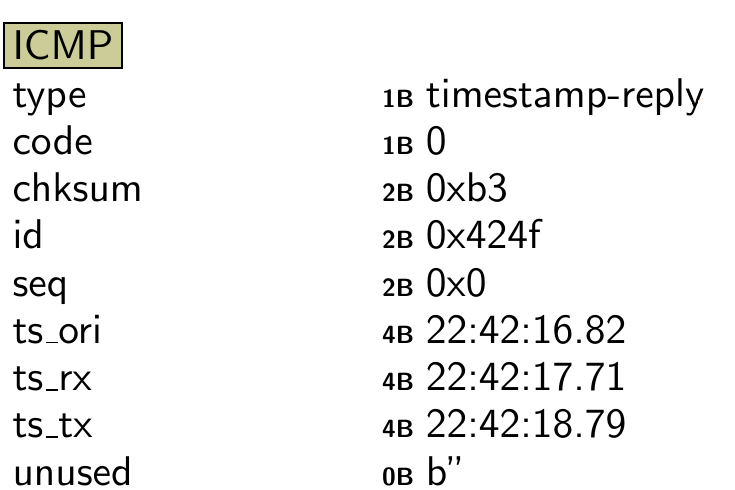
\includegraphics[width=\textwidth]{../Tesi/img/ICMP_storageCC/immagine_timestamp.png}
\captionof{figure}{Messaggio ICMP con i campi \textit{Timestamp} impostati} 
\end{columns}
\end{frame} 

%\begin{frame} [fragile] 
%\frametitle{Packet Too Big}  
%\begin{center} 
%{\scriptsize 
%\begin{bytefield}[bitwidth=1.1em]{32} 
%        %\bitbox{8}{0} & \bitbox{8}{1} & \bitbox{8}{2} & \bitbox{8}{3} \\
%        \bitheader{0-31} \\
%        \bitbox{8} {Type=2 (1 byte)} & \bitbox{8}{Code=0 (1 byte)} & \bitbox{16}{Checksum (2 byte)} \\
%        \bitbox{32} {MTU (4 byte)} \\
%        \bitbox{32} {As much of invoking packet as possible without} \\
%        \bitbox{32} {the ICMPv6 packet exceeding the minimum IPv6 MTU ($\geq$ 0 byte)} 
%\end{bytefield} 
%\captionof{figure}{Struttura del pacchetto \textbf{ICMPv6 Packet Too Big}}
%}\end{center} 
%%\justifying 
%Nel campo \textbf{MTU} viene indicata la capacità massima del collegamento. 
%L'intera dimensione del campo verrà usata per l'inserimento dei dati. 
%Questo permetterà di poter inserire \textbf{4 byte} di dati. 
%\vspace{1ex} \newline
%\end{frame} 

\begin{frame}
\frametitle{Inserimento dei dati nel campo Pointer e MTU} 
\begin{columns}[T,onlytextwidth]
\column{0.48\textwidth}   
\justifying 
Il campo \textbf{Pointer} indica l'ottetto del messaggio in 
cui è presente l'errore; tuttavia può contenere dei 
dati non correlati ad esso. Nel nostro caso, verranno 
inseriti tanti dati quanto la sua capacità. 
\column{0.48\textwidth}  
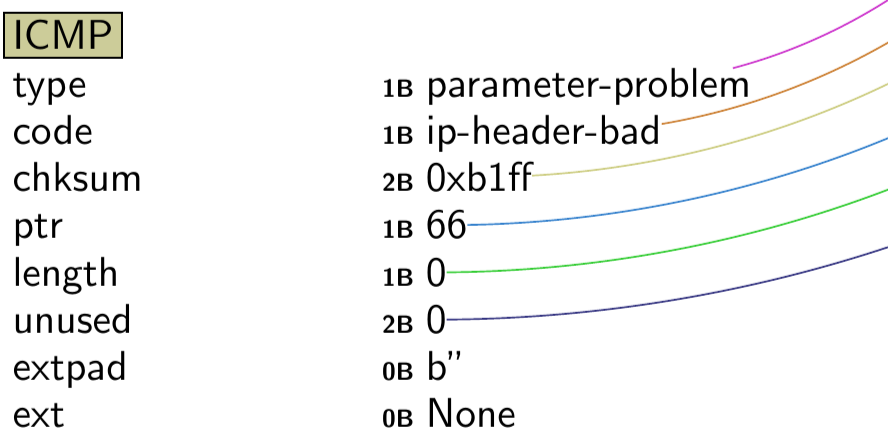
\includegraphics[width=0.8\textwidth]{../Tesi/img/ICMP_storageCC/immagine_pointer.png}
\captionof{figure}{Messaggio ICMP con campo \textit{pointer} impostato}     
\end{columns} 
Nel campo \textbf{MTU} invece viene indicata la capacità 
massima del collegamento. L'intera dimensione del 
campo verrà usata per l'inserimento dei dati. Anche 
in esso si inseriranno tanti dati quanto la sua 
capacità. 
\end{frame}  
\begin{frame} 
\frametitle{Inserimento dei dati nel campo Invoking Packet} 
Invece nel campo \textbf{Invoking Packet} verrà indicato il pacchetto che 
ha causato l'errore. Nel nostro caso si userà un pacchetto IP/ICMP. Tramite 
i campi sfruttati si riesce ad inserire \textbf{7 byte} di dati. 
\scriptsize 
\begin{longtable}{|p{0.3\textwidth}|p{0.3\textwidth}|p{0.3\textwidth}|} 
    \multicolumn{3}{c}{Header IPv6} \\ 
    \hline 
    \textbf{Campo} & \textbf{Byte} & \textbf{Utilizzo} \\
    \hline 
    Payload Length & 2 byte & Tempo di vita del pacchetto\\  
    \hline 
    %Next Header & 1 byte & Indica il tipo di header seguente a quello di IPv6 \\  
    %\hline 
    Hop Limit & 1 byte & Decrementato di 1 per ogni nodo che inoltra il pacchetto \\  
    \hline 
    \multicolumn{3}{c}{Header ICMPv6} \\
    \hline
    \textbf{Campo} & \textbf{Byte} & \textbf{Utilizzo} \\
    \hline
    Identifier & 2 byte & Identificativo del messaggio di richiesta invocato \\  
    \hline 
    Sequence & 2 byte & Numero di sequenza del messaggio di richiesta invocato \\  
    \hline 
    \caption{Struttura del campo Invoking Packet} 
    \label{table:icmpv6:invokinppacket} 
\end{longtable}
\end{frame}  
